%\VignetteEngine{knitr::knitr}
%\VignetteIndexEntry{Semi supervised Grade of Memebership models for RNA-seq data using classtpx}
%\VignettePackage{classtpx}

% To compile this document
% library('knitr'); rm(list=ls()); knit('classtpx/vignettes/classtpx-vignette.Rnw')
% library('knitr'); rm(list=ls()); knit2pdf('classtpx/vignettes/classtpx-vignette.Rnw'); openPDF('classtpx-vignette.pdf')
%

\documentclass[12pt]{article}\usepackage[]{graphicx}\usepackage[usenames,dvipsnames]{color}
%% maxwidth is the original width if it is less than linewidth
%% otherwise use linewidth (to make sure the graphics do not exceed the margin)
\makeatletter
\def\maxwidth{ %
  \ifdim\Gin@nat@width>\linewidth
    \linewidth
  \else
    \Gin@nat@width
  \fi
}
\makeatother

\definecolor{fgcolor}{rgb}{0.345, 0.345, 0.345}
\newcommand{\hlnum}[1]{\textcolor[rgb]{0.686,0.059,0.569}{#1}}%
\newcommand{\hlstr}[1]{\textcolor[rgb]{0.192,0.494,0.8}{#1}}%
\newcommand{\hlcom}[1]{\textcolor[rgb]{0.678,0.584,0.686}{\textit{#1}}}%
\newcommand{\hlopt}[1]{\textcolor[rgb]{0,0,0}{#1}}%
\newcommand{\hlstd}[1]{\textcolor[rgb]{0.345,0.345,0.345}{#1}}%
\newcommand{\hlkwa}[1]{\textcolor[rgb]{0.161,0.373,0.58}{\textbf{#1}}}%
\newcommand{\hlkwb}[1]{\textcolor[rgb]{0.69,0.353,0.396}{#1}}%
\newcommand{\hlkwc}[1]{\textcolor[rgb]{0.333,0.667,0.333}{#1}}%
\newcommand{\hlkwd}[1]{\textcolor[rgb]{0.737,0.353,0.396}{\textbf{#1}}}%

\usepackage{framed}
\makeatletter
\newenvironment{kframe}{%
 \def\at@end@of@kframe{}%
 \ifinner\ifhmode%
  \def\at@end@of@kframe{\end{minipage}}%
  \begin{minipage}{\columnwidth}%
 \fi\fi%
 \def\FrameCommand##1{\hskip\@totalleftmargin \hskip-\fboxsep
 \colorbox{shadecolor}{##1}\hskip-\fboxsep
     % There is no \\@totalrightmargin, so:
     \hskip-\linewidth \hskip-\@totalleftmargin \hskip\columnwidth}%
 \MakeFramed {\advance\hsize-\width
   \@totalleftmargin\z@ \linewidth\hsize
   \@setminipage}}%
 {\par\unskip\endMakeFramed%
 \at@end@of@kframe}
\makeatother

\definecolor{shadecolor}{rgb}{.97, .97, .97}
\definecolor{messagecolor}{rgb}{0, 0, 0}
\definecolor{warningcolor}{rgb}{1, 0, 1}
\definecolor{errorcolor}{rgb}{1, 0, 0}
\newenvironment{knitrout}{}{} % an empty environment to be redefined in TeX

\usepackage{alltt}

\newcommand{\classtpx}{\textit{classtpx}}
\newcommand\numberthis{\addtocounter{equation}{1}\tag{\theequation}}
\usepackage{dsfont}
\usepackage{cite}
\usepackage{amsmath} 





\RequirePackage{/Library/Frameworks/R.framework/Versions/3.2/Resources/library/BiocStyle/resources/tex/Bioconductor}

\AtBeginDocument{\bibliographystyle{/Library/Frameworks/R.framework/Versions/3.2/Resources/library/BiocStyle/resources/tex/unsrturl}}


\author{Kushal K Dey, Chiaowen Joyce Hsiao \& Matthew Stephens \\[1em] \small{\textit{Stephens Lab}, The University of Chicago} \mbox{ }\\ \small{\texttt{$^*$Correspondending Email: mstephens@uchicago.edu}}}

\bioctitle[Semi supervised Grade of Membership models for RNA-seq data using \classtpx{}]{Semi supervised Grade of Membership models for RNA-seq data using \classtpx{}}
\IfFileExists{upquote.sty}{\usepackage{upquote}}{}
\begin{document}

\maketitle



\newpage

\tableofcontents

\section{Introduction}

The Grade of Membership (GoM) model, as fitted by the \begin{verb} topics() \end{verb} function of the package \CRANpkg{maptpx} or the \begin{verb} FitGoM() \end{verb} in the package CountClust, suffers from the issue of identifiability, the reason being clusters that are determined in a completely unsupervised way. Oftentimes, we may have information about expression patterns of the biological clusters of interest. To cite an example, suppose we have RNA-seq data on blood samples (bulk or single cell) and also RNA-seq data on some FACS sorted single cells from Blood identifying different Blood cell types. Sequencing these FACS sorted cells gives us information of the expression patterns of the underlying cell types. One can view these cell types as potential clusters in clustering of RNA-seq data (non FACS sorted) from Blood. It is this prior information about the clusters that can ultimately lead to more distinct patterns of expression compared to unsupervised models and give a better sense about the mixing proportions of different cell types of interest in the samples.

\section{Installation}

To install the current working version of the \classtpx{} package, make sure FORTRAN compatibility.

\begin{knitrout}
\definecolor{shadecolor}{rgb}{0.969, 0.969, 0.969}\color{fgcolor}\begin{kframe}
\begin{alltt}
\hlcom{#curl -O http://r.research.att.com/libs/gfortran-4.8.2-darwin13.tar.bz2}
\hlcom{#sudo tar fvxz gfortran-4.8.2-darwin13.tar.bz2 -C /}
\end{alltt}
\end{kframe}
\end{knitrout}

To install the Github working version,

\begin{knitrout}
\definecolor{shadecolor}{rgb}{0.969, 0.969, 0.969}\color{fgcolor}\begin{kframe}
\begin{alltt}
\hlstd{devtools}\hlopt{::}\hlkwd{install_github}\hlstd{(}\hlstr{"kkdey/classtpx"}\hlstd{)}
\end{alltt}
\end{kframe}
\end{knitrout}

To load the package

\begin{knitrout}
\definecolor{shadecolor}{rgb}{0.969, 0.969, 0.969}\color{fgcolor}\begin{kframe}
\begin{alltt}
\hlkwd{library}\hlstd{(}\hlstr{"classtpx"}\hlstd{)}
\end{alltt}
\end{kframe}
\end{knitrout}



\section{Data Preparation}

Recently a number of studies have been published on FACS sorted RNA-sequqnicng data with the aim of identifying distinct cell types of cell cycle phases. We are trying to build a library of data packages that seem relevant to our research interest and have them available as ExpressionSet objects (integrating the expression data succinctly with metadata information on samples and features). You can find a number of these data packages hosted on our Github pages \url{https://github.com/kkdey?tab=repositories} and \url{https://github.com/jhsiao999?tab=repositories}.

We present an example of the Leng et al 2015 data [paper site: \url{http://www.nature.com/nmeth/journal/v12/n10/full/nmeth.3549.html}] of RNA-sequencing data on human embryonic stem cells. Total 213 H1 single cells and 247 H1-Fucci single cells were sequenced. The 213 H1 cells were used to evaluate Oscope in identifying oscillatory genes. The H1-Fucci cells were used to confirm the cell cycle gene cluster identified by Oscope in the H1 hESCs. In the dataset, we had cells labeled H1 (213), G1 (91), S (80) and G2 (76).


\begin{knitrout}
\definecolor{shadecolor}{rgb}{0.969, 0.969, 0.969}\color{fgcolor}\begin{kframe}
\begin{alltt}
\hlstd{devtools}\hlopt{::}\hlkwd{install_github}\hlstd{(}\hlstr{"kkdey/singleCellRNASeqHumanLengESC"}\hlstd{,} \hlkwc{force}\hlstd{=}\hlnum{TRUE}\hlstd{)}
\end{alltt}
\end{kframe}
\end{knitrout}

\begin{knitrout}
\definecolor{shadecolor}{rgb}{0.969, 0.969, 0.969}\color{fgcolor}\begin{kframe}
\begin{alltt}
\hlkwd{library}\hlstd{(singleCellRNASeqHumanLengESC)}
\hlkwd{data}\hlstd{(}\hlstr{"HumanLengESC"}\hlstd{)}
\hlstd{leng_gene_names} \hlkwb{<-} \hlstd{Biobase}\hlopt{::}\hlkwd{featureNames}\hlstd{(HumanLengESC);}

\hlstd{leng_data} \hlkwb{<-} \hlkwd{t}\hlstd{(Biobase}\hlopt{::}\hlkwd{exprs}\hlstd{(HumanLengESC));}
\hlstd{leng_metadata} \hlkwb{<-} \hlstd{Biobase}\hlopt{::}\hlkwd{pData}\hlstd{(HumanLengESC)}
\hlstd{leng_cell_state} \hlkwb{<-} \hlstd{leng_metadata}\hlopt{$}\hlstd{cell_state;}

\hlkwd{table}\hlstd{(leng_cell_state)}
\end{alltt}
\begin{verbatim}
## leng_cell_state
##  G1  G2  H1   S 
##  91  76 213  80
\end{verbatim}
\end{kframe}
\end{knitrout}

\section{Methods and Materials}

The general framework for Grade of Membership (GoM) models is as follows.

suppose $c_{ng}$ represents the read counts for sample $n$ and gene $g$. Then we assume the model

\begin{equation}
\left (c_{n1}, c_{n2}, \cdots, c_{nG} \right) \sim Mult \left (c_{n+}, p_{n1}, p_{n2}, \cdots, p_{nG} \right)
\end{equation}

where $p_{ng}$ represents the probability of observing a read mapping to gene $g$ from sample $n$. We write this probability as 

\begin{equation}
p_{ng} = \sum_{k=1}^{K} \omega_{nk} \theta_{kg} \hspace{1 cm} \sum_{k=1}^{K} \omega_{nk}=1 \hspace{0.5 cm} \forall n \hspace{1 cm} \sum_{g=1}^{G} \theta_{kg}=1 \hspace{0.5 cm} \forall k 
\end{equation}

where $\omega_{nk}$ represents membership probability of $k$ th cluster in the $n$ th sample and $\theta_{kg}$ represents cluster mass at gene $g$ for cluster $k$.

In standard GoM models, the priors on $\omega$ and $\theta$ are non-informative.

\begin{equation}
\left(\omega_{n1}, \omega_{n2}, \cdots, \omega_{nK} \right) \sim Dir \left ( \frac{1}{K}, \frac{1}{K}, \cdots, \frac{1}{K} \right)
\end{equation}

\begin{equation}
\left(\theta_{k1}, \theta_{k2}, \cdots, \theta_{kG} \right) \sim Dir \left ( \frac{1}{KG}, \frac{1}{KG}, \cdots, \frac{1}{KG} \right)
\end{equation}

Now in \classtpx{}, we assume that for some samples, the class labels or cluster labels are known. 
This information is used to either drive the $\theta$ matrix or the $\omega$ matrix. For instance, in the Leng et al 2015 data, the three classes may be considered to be the G1, S and G2 phases. There are three methods we propose 

\begin{itemize}

\item \textbf{omega.fix}: We fix the $\omega$ vector for the samples for which the class labels are known. For instance, in the Leng et al 2015 data, for a classtpx model with K=3 representing the clusters due to G1, S and G2 phases, if the sample $n$ comes from the G1 phase, we fix $\omega_{n.} = (1,0,0)$. Similarly, if the sample comes from S or G2 phase, we fix $\omega_{n.}$ to be $(0,1,0)$ and $(0,0,1)$ respectively. For the cells corresponding to H1 phase, the $\omega$ vector is not known and estimated from the data. In mathematical terms, we can write the model for $\omega$ as follows 

\begin{align*}
\left(\omega_{n1}, \omega_{n2}, \cdots, \omega_{nK} \right) & = e_{k} \hspace{1 cm} if \hspace{0.5 cm} class(n) = k  \\
\left(\omega_{n1}, \omega_{n2}, \cdots, \omega_{nK} \right) & \sim Dir \left ( \frac{1}{K}, \frac{1}{K}, \cdots, \frac{1}{K} \right) \hspace{1 cm} if \hspace{0.5 cm} class(n) = NULL \\
\end{align*}

where $class(n)$ represents the class label of the sample (it is NULL if the class label is not known). $e_{k}$ is the vector with $1$ at position $k$ and $0$ at all other positions of the vector. We then perform updates on the $\omega$ on the NULL class label samples and the $\theta$ matrix and the updating scheme is similar to the \begin{verb} topics() \end{verb} as in \CRANpkg{maptpx} package due to Matt Taddy.

\item \textbf{theta.prior}: For each class label $k$, we pool all samples $n$ with $class(n)=k$, and then normalize the counts data to determine the prior $\theta$ matrix.

\begin{align*}
\theta_{kg} & = \frac{\sum_{n:class(n)=k} c_{ng}}{\sum_{g} \sum_{n:class(n)=k} c_{ng}} \hspace{0.5 cm} \forall g,  \hspace{0.5 cm} if \hspace{0.5 cm} card \{n: class(n)=k \} \neq 0 \nonumber \\
\left(\theta_{k1}, \theta_{k2}, \cdots, \theta_{kG} \right) & \sim Dir \left ( \frac{1}{KG}, \frac{1}{KG}, \cdots, \frac{1}{KG} \right) \hspace{0.5 cm} if \hspace{0.5 cm} card \{n: class(n)=k \}= 0  \numberthis \label{eq:eq1} \\
\end{align*}

One can also apply adaptive shrinkage on the $\theta_{k.}$ values. In that case, define

\begin{equation}
\beta_{kg} = \frac{\sum_{n:class(n)=k} c_{ng}}{N_{k}} - \frac{\sum_{g} \sum_{n:class(n)=k} c_{ng}}{N} \hspace{0.5 cm}  card \{n: class(n)=k \}=N_{k}
\end{equation}

We assume

\begin{equation}
s_{kg} = \frac{1}{N_{k} (N_{k}-1)} \sum_{class(n)=k} \left (c_{ng} - \frac{\sum_{n:class(n)=k} c_{ng}}{N_{k}} \right )^{2} \hspace{0.5 cm} card \{n: class(n)=k \}=N_{k}
\end{equation}

Then we perform \begin{verb} ash \end{verb} on the vector $(\beta_{kg}, s_{kg})$ over all genes $g$ for each $k$ and then obtain the posterior mean of $\beta$, say $\beta_{post}(kg)$.

We then fix the $\theta$ values as 

\begin{equation}
\theta^{\star}_{kg} = \frac{\sum_{g} \sum_{n:class(n)=k} c_{ng}}{N} + \beta_{post}(kg)
\end{equation}

So, in other words we assume

\begin{align*}
\theta_{kg} & = \theta^{\star}_{kg} \hspace{0.5 cm} \forall g,  \hspace{0.5 cm} if \hspace{0.5 cm} card \{n: class(n)=k \} \neq 0 \nonumber \\
\left(\theta_{k1}, \theta_{k2}, \cdots, \theta_{kG} \right) & \sim Dir \left ( \frac{1}{KG}, \frac{1}{KG}, \cdots, \frac{1}{KG} \right) \hspace{0.5 cm} if \hspace{0.5 cm} card \{n: class(n)=k \}= 0 \numberthis \label{eq:eq2} \\
\end{align*}

These $\theta_{k.}$ as in Eqn \eqref{eq:eq1} or Eqn \eqref{eq:eq2} (depending on whether we use shrinkage or not) are then input into the GoM model framework as prior cluster probability vectors and we update them based on the data to find the posterior estimates at each stage of iteration (the updating scheme similar to the \begin{verb} topics() \end{verb} as in \CRANpkg{maptpx} package due to Matt Taddy).

\item \textbf{theta.fix}: In this method, instead of setting $\theta_{k.}$ matrix for $k$ with $N_{k} \neq 0$ as prior, we fix them at these values and do not update them during the iterative steps. The only updates correspond to those $k$ for which $N_{k} = 0$, and the updating scheme is similar to the \begin{verb} topics() \end{verb} as in \CRANpkg{maptpx} package due to Matt Taddy.
\end{itemize}

\section{Results}

We first cite the example of the Leng et al data and fit \begin{verb} classtpx() \end{verb} model on the data. 

\subsection{Leng et al (2015)}

We fix the class labels and the sample indices as follows.

\begin{knitrout}
\definecolor{shadecolor}{rgb}{0.969, 0.969, 0.969}\color{fgcolor}\begin{kframe}
\begin{alltt}
\hlstd{index_1} \hlkwb{<-} \hlkwd{which}\hlstd{(leng_cell_state}\hlopt{==}\hlstr{"G1"}\hlstd{);}
\hlstd{index_2} \hlkwb{<-} \hlkwd{which}\hlstd{(leng_cell_state}\hlopt{==}\hlstr{"S"}\hlstd{);}
\hlstd{index_3} \hlkwb{<-} \hlkwd{which}\hlstd{(leng_cell_state}\hlopt{==}\hlstr{"G2"}\hlstd{);}

\hlstd{known_samples} \hlkwb{<-} \hlkwd{c}\hlstd{(index_1, index_2, index_3);}
\hlstd{class_labs} \hlkwb{<-} \hlkwd{c}\hlstd{(}\hlkwd{rep}\hlstd{(}\hlstr{"G1"}\hlstd{,} \hlkwd{length}\hlstd{(index_1)),}
                \hlkwd{rep}\hlstd{(}\hlstr{"S"}\hlstd{,} \hlkwd{length}\hlstd{(index_2)),}
                \hlkwd{rep}\hlstd{(}\hlstr{"G2"}\hlstd{,} \hlkwd{length}\hlstd{(index_3)));}
\end{alltt}
\end{kframe}
\end{knitrout}

Then we can perform \begin{verb} classtpx() \end{verb} model for \begin{verb} omega.fix() \end{verb} method as follows 

\begin{knitrout}
\definecolor{shadecolor}{rgb}{0.969, 0.969, 0.969}\color{fgcolor}\begin{kframe}
\begin{alltt}
\hlstd{Topic_clus} \hlkwb{<-} \hlstd{classtpx}\hlopt{::}\hlkwd{class_topics}\hlstd{(}
    \hlstd{leng_data,}
    \hlkwc{K}\hlstd{=}\hlnum{3}\hlstd{,}
    \hlkwc{known_samples} \hlstd{= known_samples,}
    \hlkwc{class_labs} \hlstd{= class_labs,}
    \hlkwc{method}\hlstd{=}\hlstr{"omega.fix"}\hlstd{,}
    \hlkwc{tol}\hlstd{=}\hlnum{0.01}\hlstd{)}

\hlkwd{save}\hlstd{(Topic_clus,} \hlkwc{file}\hlstd{=}\hlstr{"../data/leng_topic_fit_3_classtpx_omega_fix.rda"}\hlstd{)}
\end{alltt}
\end{kframe}
\end{knitrout}

We can perform Structure plot visualization of the results.

\begin{knitrout}
\definecolor{shadecolor}{rgb}{0.969, 0.969, 0.969}\color{fgcolor}\begin{kframe}
\begin{alltt}
\hlstd{Topic_clus} \hlkwb{<-} \hlkwd{get}\hlstd{(}\hlkwd{load}\hlstd{(}\hlkwc{file}\hlstd{=}\hlstr{"../data/leng_topic_fit_3_classtpx_omega_fix.rda"}\hlstd{))}

\hlstd{omega} \hlkwb{<-} \hlstd{Topic_clus}\hlopt{$}\hlstd{omega;}

\hlstd{annotation} \hlkwb{<-} \hlkwd{data.frame}\hlstd{(}
  \hlkwc{sample_id} \hlstd{=} \hlkwd{paste0}\hlstd{(}\hlstr{"X"}\hlstd{,} \hlkwd{c}\hlstd{(}\hlnum{1}\hlopt{:}\hlkwd{NROW}\hlstd{(omega))),}
  \hlkwc{tissue_label} \hlstd{=} \hlkwd{factor}\hlstd{(leng_cell_state,}
                        \hlkwc{levels} \hlstd{=} \hlkwd{c}\hlstd{(}\hlstr{"G1"}\hlstd{,} \hlstr{"S"}\hlstd{,} \hlstr{"G2"}\hlstd{,} \hlstr{"H1"}\hlstd{) ) )}


\hlkwd{rownames}\hlstd{(omega)} \hlkwb{<-} \hlstd{annotation}\hlopt{$}\hlstd{sample_id;}


\hlstd{CountClust}\hlopt{::}\hlkwd{StructureGGplot}\hlstd{(}\hlkwc{omega} \hlstd{= omega,}
                \hlkwc{annotation} \hlstd{= annotation,}
                \hlkwc{palette} \hlstd{= RColorBrewer}\hlopt{::}\hlkwd{brewer.pal}\hlstd{(}\hlnum{8}\hlstd{,} \hlstr{"Accent"}\hlstd{),}
                \hlkwc{yaxis_label} \hlstd{=} \hlstr{"Cell cycle phase"}\hlstd{,}
                \hlkwc{order_sample} \hlstd{=} \hlnum{TRUE}\hlstd{,}
                \hlkwc{axis_tick} \hlstd{=} \hlkwd{list}\hlstd{(}\hlkwc{axis_ticks_length} \hlstd{=} \hlnum{.1}\hlstd{,}
                                 \hlkwc{axis_ticks_lwd_y} \hlstd{=} \hlnum{.1}\hlstd{,}
                                 \hlkwc{axis_ticks_lwd_x} \hlstd{=} \hlnum{.1}\hlstd{,}
                                 \hlkwc{axis_label_size} \hlstd{=} \hlnum{7}\hlstd{,}
                                 \hlkwc{axis_label_face} \hlstd{=} \hlstr{"bold"}\hlstd{))}
\end{alltt}
\end{kframe}
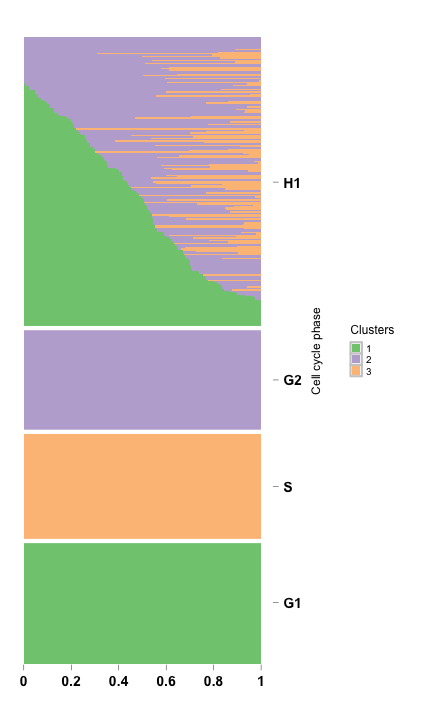
\includegraphics[width=3 in,height=5 in]{figure/structure_leng_1-1} 

\end{knitrout}

We now perform  \begin{verb} classtpx() \end{verb} model for \begin{verb} theta.prior() \end{verb} method.

\begin{knitrout}
\definecolor{shadecolor}{rgb}{0.969, 0.969, 0.969}\color{fgcolor}\begin{kframe}
\begin{alltt}
\hlstd{Topic_clus} \hlkwb{<-} \hlstd{classtpx}\hlopt{::}\hlkwd{class_topics}\hlstd{(}
    \hlstd{leng_data,}
    \hlkwc{K}\hlstd{=}\hlnum{3}\hlstd{,}
    \hlkwc{known_samples} \hlstd{= known_samples,}
    \hlkwc{class_labs} \hlstd{= class_labs,}
    \hlkwc{method}\hlstd{=}\hlstr{"theta.prior"}\hlstd{,}
    \hlkwc{tol}\hlstd{=}\hlnum{0.01}\hlstd{,}
    \hlkwc{shrink}\hlstd{=}\hlnum{TRUE}\hlstd{)}

\hlkwd{save}\hlstd{(Topic_clus,} \hlkwc{file}\hlstd{=}\hlstr{"../data/leng_topic_fit_3_classtpx_theta_prior.rda"}\hlstd{)}
\end{alltt}
\end{kframe}
\end{knitrout}

We can perform Structure plot visualization of the results.

\begin{knitrout}
\definecolor{shadecolor}{rgb}{0.969, 0.969, 0.969}\color{fgcolor}\begin{kframe}
\begin{alltt}
\hlstd{Topic_clus} \hlkwb{<-} \hlkwd{get}\hlstd{(}\hlkwd{load}\hlstd{(}\hlkwc{file}\hlstd{=}\hlstr{"../data/leng_topic_fit_3_classtpx_theta_prior.rda"}\hlstd{))}

\hlstd{omega} \hlkwb{<-} \hlstd{Topic_clus}\hlopt{$}\hlstd{omega;}

\hlstd{annotation} \hlkwb{<-} \hlkwd{data.frame}\hlstd{(}
  \hlkwc{sample_id} \hlstd{=} \hlkwd{paste0}\hlstd{(}\hlstr{"X"}\hlstd{,} \hlkwd{c}\hlstd{(}\hlnum{1}\hlopt{:}\hlkwd{NROW}\hlstd{(omega))),}
  \hlkwc{tissue_label} \hlstd{=} \hlkwd{factor}\hlstd{(leng_cell_state,}
                        \hlkwc{levels} \hlstd{=} \hlkwd{c}\hlstd{(}\hlstr{"G1"}\hlstd{,} \hlstr{"S"}\hlstd{,} \hlstr{"G2"}\hlstd{,} \hlstr{"H1"}\hlstd{) ) )}


\hlkwd{rownames}\hlstd{(omega)} \hlkwb{<-} \hlstd{annotation}\hlopt{$}\hlstd{sample_id;}


\hlstd{CountClust}\hlopt{::}\hlkwd{StructureGGplot}\hlstd{(}\hlkwc{omega} \hlstd{= omega,}
                \hlkwc{annotation} \hlstd{= annotation,}
                \hlkwc{palette} \hlstd{= RColorBrewer}\hlopt{::}\hlkwd{brewer.pal}\hlstd{(}\hlnum{8}\hlstd{,} \hlstr{"Accent"}\hlstd{),}
                \hlkwc{yaxis_label} \hlstd{=} \hlstr{"Cell cycle phase"}\hlstd{,}
                \hlkwc{order_sample} \hlstd{=} \hlnum{TRUE}\hlstd{,}
                \hlkwc{axis_tick} \hlstd{=} \hlkwd{list}\hlstd{(}\hlkwc{axis_ticks_length} \hlstd{=} \hlnum{.1}\hlstd{,}
                                 \hlkwc{axis_ticks_lwd_y} \hlstd{=} \hlnum{.1}\hlstd{,}
                                 \hlkwc{axis_ticks_lwd_x} \hlstd{=} \hlnum{.1}\hlstd{,}
                                 \hlkwc{axis_label_size} \hlstd{=} \hlnum{7}\hlstd{,}
                                 \hlkwc{axis_label_face} \hlstd{=} \hlstr{"bold"}\hlstd{))}
\end{alltt}
\end{kframe}
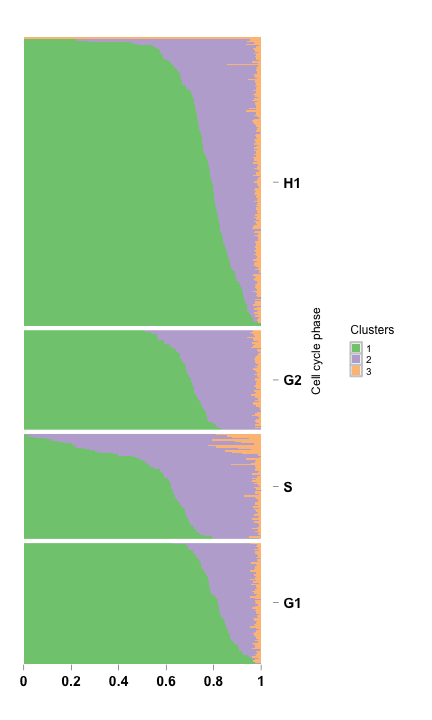
\includegraphics[width=3 in,height=5 in]{figure/structure_leng_2-1} 

\end{knitrout}

Finally we apply the \begin{verb} theta.fix() \end{verb} method.

\begin{knitrout}
\definecolor{shadecolor}{rgb}{0.969, 0.969, 0.969}\color{fgcolor}\begin{kframe}
\begin{alltt}
\hlstd{Topic_clus} \hlkwb{<-} \hlstd{classtpx}\hlopt{::}\hlkwd{class_topics}\hlstd{(}
    \hlstd{leng_data,}
    \hlkwc{K}\hlstd{=}\hlnum{3}\hlstd{,}
    \hlkwc{known_samples} \hlstd{= known_samples,}
    \hlkwc{class_labs} \hlstd{= class_labs,}
    \hlkwc{method}\hlstd{=}\hlstr{"theta.fix"}\hlstd{,}
    \hlkwc{tol}\hlstd{=}\hlnum{0.01}\hlstd{,}
    \hlkwc{shrink}\hlstd{=}\hlnum{FALSE}\hlstd{)}

\hlkwd{save}\hlstd{(Topic_clus,} \hlkwc{file}\hlstd{=}\hlstr{"../data/leng_topic_fit_3_classtpx_theta_fix.rda"}\hlstd{)}
\end{alltt}
\end{kframe}
\end{knitrout}

We can perform Structure plot visualization of the results.

\begin{knitrout}
\definecolor{shadecolor}{rgb}{0.969, 0.969, 0.969}\color{fgcolor}\begin{kframe}
\begin{alltt}
\hlstd{Topic_clus} \hlkwb{<-} \hlkwd{get}\hlstd{(}\hlkwd{load}\hlstd{(}\hlkwc{file}\hlstd{=}\hlstr{"../data/leng_topic_fit_3_classtpx_theta_fix.rda"}\hlstd{))}

\hlstd{omega} \hlkwb{<-} \hlstd{Topic_clus}\hlopt{$}\hlstd{omega;}

\hlstd{annotation} \hlkwb{<-} \hlkwd{data.frame}\hlstd{(}
  \hlkwc{sample_id} \hlstd{=} \hlkwd{paste0}\hlstd{(}\hlstr{"X"}\hlstd{,} \hlkwd{c}\hlstd{(}\hlnum{1}\hlopt{:}\hlkwd{NROW}\hlstd{(omega))),}
  \hlkwc{tissue_label} \hlstd{=} \hlkwd{factor}\hlstd{(leng_cell_state,}
                        \hlkwc{levels} \hlstd{=} \hlkwd{c}\hlstd{(}\hlstr{"G1"}\hlstd{,} \hlstr{"S"}\hlstd{,} \hlstr{"G2"}\hlstd{,} \hlstr{"H1"}\hlstd{) ) )}


\hlkwd{rownames}\hlstd{(omega)} \hlkwb{<-} \hlstd{annotation}\hlopt{$}\hlstd{sample_id;}


\hlstd{CountClust}\hlopt{::}\hlkwd{StructureGGplot}\hlstd{(}\hlkwc{omega} \hlstd{= omega,}
                \hlkwc{annotation} \hlstd{= annotation,}
                \hlkwc{palette} \hlstd{= RColorBrewer}\hlopt{::}\hlkwd{brewer.pal}\hlstd{(}\hlnum{8}\hlstd{,} \hlstr{"Accent"}\hlstd{),}
                \hlkwc{yaxis_label} \hlstd{=} \hlstr{"Cell cycle phase"}\hlstd{,}
                \hlkwc{order_sample} \hlstd{=} \hlnum{TRUE}\hlstd{,}
                \hlkwc{axis_tick} \hlstd{=} \hlkwd{list}\hlstd{(}\hlkwc{axis_ticks_length} \hlstd{=} \hlnum{.1}\hlstd{,}
                                 \hlkwc{axis_ticks_lwd_y} \hlstd{=} \hlnum{.1}\hlstd{,}
                                 \hlkwc{axis_ticks_lwd_x} \hlstd{=} \hlnum{.1}\hlstd{,}
                                 \hlkwc{axis_label_size} \hlstd{=} \hlnum{7}\hlstd{,}
                                 \hlkwc{axis_label_face} \hlstd{=} \hlstr{"bold"}\hlstd{))}
\end{alltt}
\end{kframe}
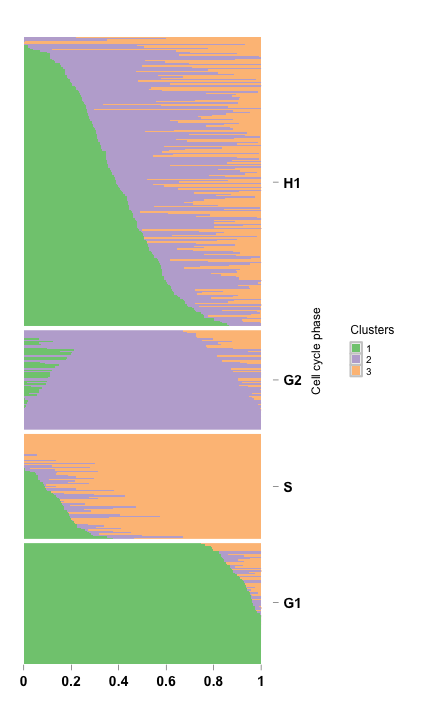
\includegraphics[width=3 in,height=5 in]{figure/structure_leng_3-1} 

\end{knitrout}

\subsection{Treutlin et al (2014)}

Treutlin et al 2014 sequenced single cell transcriptome data from mouse lung epithelium. The cells were collected at various stages E14.5, E16.5, E18.5 and some adult replicates. We performed both \begin{verb} maptpx() \end{verb} model and \begin{verb} classtpx \end{verb} model fitting on this data.

\begin{knitrout}
\definecolor{shadecolor}{rgb}{0.969, 0.969, 0.969}\color{fgcolor}\begin{kframe}
\begin{alltt}
\hlstd{devtools}\hlopt{::}\hlkwd{install_github}\hlstd{(}\hlstr{"jhsiao999/singleCellRNASeqMouseTreutleinLung"}\hlstd{,} \hlkwc{force}\hlstd{=}\hlnum{TRUE}\hlstd{)}
\end{alltt}
\end{kframe}
\end{knitrout}

\begin{knitrout}
\definecolor{shadecolor}{rgb}{0.969, 0.969, 0.969}\color{fgcolor}\begin{kframe}
\begin{alltt}
\hlkwd{library}\hlstd{(singleCellRNASeqMouseTreutleinLung)}
\hlkwd{data}\hlstd{(}\hlstr{"MouseTreutleinLung"}\hlstd{)}
\hlstd{leng_gene_names} \hlkwb{<-} \hlstd{Biobase}\hlopt{::}\hlkwd{featureNames}\hlstd{(HumanLengESC);}

\hlstd{counts_data} \hlkwb{<-} \hlkwd{t}\hlstd{(Biobase}\hlopt{::}\hlkwd{exprs}\hlstd{(MouseTreutleinLung));}
\hlstd{pheno_metadata} \hlkwb{<-} \hlkwd{pData}\hlstd{(MouseTreutleinLung);}
\hlkwd{table}\hlstd{(pheno_metadata[,}\hlnum{1}\hlstd{])}
\end{alltt}
\begin{verbatim}
## 
## adult E14.5 E16.5 E18.5 
##    46    45    27    83
\end{verbatim}
\end{kframe}
\end{knitrout}

We first apply the maptpx model for $K=3$.

\begin{knitrout}
\definecolor{shadecolor}{rgb}{0.969, 0.969, 0.969}\color{fgcolor}\begin{kframe}
\begin{alltt}
\hlstd{Topic_clus} \hlkwb{<-} \hlstd{maptpx}\hlopt{::}\hlkwd{topics}\hlstd{(counts_data,} \hlnum{3}\hlstd{,} \hlkwc{tol}\hlstd{=}\hlnum{0.1}\hlstd{);}
\hlkwd{save}\hlstd{(Topic_clus,} \hlkwc{file}\hlstd{=}\hlstr{"../data/treutlin_topic_fit_3_maptpx.rda"}\hlstd{)}
\end{alltt}
\end{kframe}
\end{knitrout}

\begin{knitrout}
\definecolor{shadecolor}{rgb}{0.969, 0.969, 0.969}\color{fgcolor}\begin{kframe}
\begin{alltt}
\hlstd{Topic_clus} \hlkwb{<-} \hlkwd{get}\hlstd{(}\hlkwd{load}\hlstd{(}\hlkwc{file}\hlstd{=}\hlstr{"../data/treutlin_topic_fit_3_maptpx.rda"}\hlstd{))}

\hlstd{omega} \hlkwb{<-} \hlstd{Topic_clus}\hlopt{$}\hlstd{omega;}

\hlstd{annotation} \hlkwb{<-} \hlkwd{data.frame}\hlstd{(}
  \hlkwc{sample_id} \hlstd{=} \hlkwd{paste0}\hlstd{(}\hlstr{"X"}\hlstd{,} \hlkwd{c}\hlstd{(}\hlnum{1}\hlopt{:}\hlkwd{NROW}\hlstd{(omega))),}
  \hlkwc{tissue_label} \hlstd{=} \hlkwd{factor}\hlstd{(}\hlkwd{paste0}\hlstd{(pheno_metadata}\hlopt{$}\hlstd{cell_type,} \hlstr{"_"}\hlstd{,}
                               \hlstd{pheno_metadata}\hlopt{$}\hlstd{replicate),}
                        \hlkwc{levels}\hlstd{=}\hlkwd{rev}\hlstd{(}\hlkwd{c}\hlstd{(}\hlstr{"E14.5_1"}\hlstd{,} \hlstr{"E16.5_1"}\hlstd{,}
                                     \hlstr{"E18.5_1"}\hlstd{,}\hlstr{"E18.5_2"}\hlstd{,}
                                     \hlstr{"E18.5_3"}\hlstd{,}\hlstr{"adult_replicate"}\hlstd{))}
\hlstd{))}

\hlkwd{rownames}\hlstd{(omega)} \hlkwb{<-} \hlstd{annotation}\hlopt{$}\hlstd{sample_id;}


\hlstd{CountClust}\hlopt{::}\hlkwd{StructureGGplot}\hlstd{(}\hlkwc{omega} \hlstd{= omega,}
                \hlkwc{annotation} \hlstd{= annotation,}
                \hlkwc{palette} \hlstd{= RColorBrewer}\hlopt{::}\hlkwd{brewer.pal}\hlstd{(}\hlnum{8}\hlstd{,} \hlstr{"Accent"}\hlstd{),}
                \hlkwc{yaxis_label} \hlstd{=} \hlstr{"Cell cycle phase"}\hlstd{,}
                \hlkwc{order_sample} \hlstd{=} \hlnum{TRUE}\hlstd{,}
                \hlkwc{axis_tick} \hlstd{=} \hlkwd{list}\hlstd{(}\hlkwc{axis_ticks_length} \hlstd{=} \hlnum{.1}\hlstd{,}
                                 \hlkwc{axis_ticks_lwd_y} \hlstd{=} \hlnum{.1}\hlstd{,}
                                 \hlkwc{axis_ticks_lwd_x} \hlstd{=} \hlnum{.1}\hlstd{,}
                                 \hlkwc{axis_label_size} \hlstd{=} \hlnum{7}\hlstd{,}
                                 \hlkwc{axis_label_face} \hlstd{=} \hlstr{"bold"}\hlstd{))}
\end{alltt}
\end{kframe}
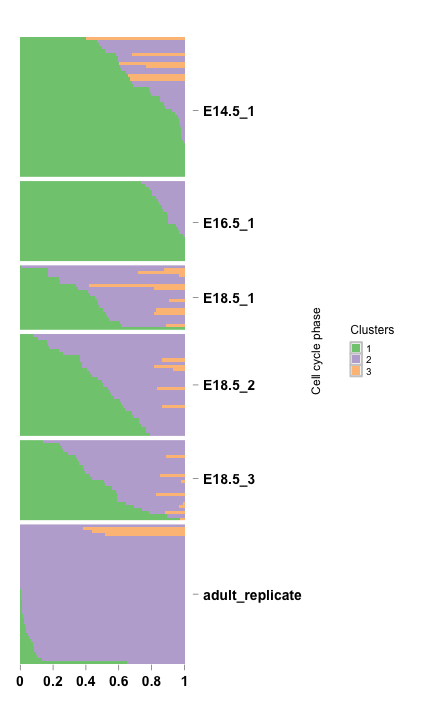
\includegraphics[width=3 in,height=5 in]{figure/structure_treutlin_maptpx-1} 

\end{knitrout}

We next performed classtpx model for K=2  with \begin{verb} omega.fix() \end{verb} method.
We chose E14.5 as one group and adult replicates as another group in defining class labels and
assumed we do not have class label information for E16.5 and E18.5 phases.

\begin{knitrout}
\definecolor{shadecolor}{rgb}{0.969, 0.969, 0.969}\color{fgcolor}\begin{kframe}
\begin{alltt}
\hlstd{known_samples} \hlkwb{<-} \hlkwd{c}\hlstd{(}\hlkwd{which}\hlstd{(pheno_metadata}\hlopt{$}\hlstd{cell_type}\hlopt{==}\hlstr{"E14.5"}\hlstd{),}
                   \hlkwd{which}\hlstd{(pheno_metadata}\hlopt{$}\hlstd{cell_type}\hlopt{==}\hlstr{"adult"}\hlstd{));}
\hlstd{class_labs} \hlkwb{<-} \hlkwd{c}\hlstd{(}\hlkwd{rep}\hlstd{(}\hlnum{1}\hlstd{,} \hlkwd{length}\hlstd{(}\hlkwd{which}\hlstd{(pheno_metadata}\hlopt{$}\hlstd{cell_type}\hlopt{==}\hlstr{"E14.5"}\hlstd{))),}
                \hlkwd{rep}\hlstd{(}\hlnum{2}\hlstd{,}\hlkwd{length}\hlstd{(}\hlkwd{which}\hlstd{(pheno_metadata}\hlopt{$}\hlstd{cell_type}\hlopt{==}\hlstr{"adult"}\hlstd{))));}
\end{alltt}
\end{kframe}
\end{knitrout}

\begin{knitrout}
\definecolor{shadecolor}{rgb}{0.969, 0.969, 0.969}\color{fgcolor}\begin{kframe}
\begin{alltt}
\hlstd{Topic_clus} \hlkwb{<-} \hlstd{classtpx}\hlopt{::}\hlkwd{class_topics}\hlstd{(}
    \hlstd{counts_data,}
    \hlkwc{K}\hlstd{=}\hlnum{2}\hlstd{,}
    \hlkwc{known_samples} \hlstd{= known_samples,}
    \hlkwc{class_labs} \hlstd{= class_labs,}
    \hlkwc{method}\hlstd{=}\hlstr{"omega.fix"}\hlstd{,}
    \hlkwc{tol}\hlstd{=}\hlnum{0.01}\hlstd{,}
    \hlkwc{shrink}\hlstd{=}\hlnum{FALSE}\hlstd{)}

\hlkwd{save}\hlstd{(Topic_clus,} \hlkwc{file}\hlstd{=}\hlstr{"../rdas/treutlin_topic_fit_2_classtpx_omega_fix.rda"}\hlstd{)}
\end{alltt}
\end{kframe}
\end{knitrout}

\begin{knitrout}
\definecolor{shadecolor}{rgb}{0.969, 0.969, 0.969}\color{fgcolor}\begin{kframe}
\begin{alltt}
\hlstd{Topic_clus} \hlkwb{<-} \hlkwd{get}\hlstd{(}\hlkwd{load}\hlstd{(}\hlkwc{file}\hlstd{=}\hlstr{"../data/treutlin_topic_fit_2_classtpx_omega_fix.rda"}\hlstd{))}

\hlstd{omega} \hlkwb{<-} \hlstd{Topic_clus}\hlopt{$}\hlstd{omega;}

\hlstd{annotation} \hlkwb{<-} \hlkwd{data.frame}\hlstd{(}
  \hlkwc{sample_id} \hlstd{=} \hlkwd{paste0}\hlstd{(}\hlstr{"X"}\hlstd{,} \hlkwd{c}\hlstd{(}\hlnum{1}\hlopt{:}\hlkwd{NROW}\hlstd{(omega))),}
  \hlkwc{tissue_label} \hlstd{=} \hlkwd{factor}\hlstd{(}\hlkwd{paste0}\hlstd{(pheno_metadata}\hlopt{$}\hlstd{cell_type,} \hlstr{"_"}\hlstd{,}
                               \hlstd{pheno_metadata}\hlopt{$}\hlstd{replicate),}
                        \hlkwc{levels}\hlstd{=}\hlkwd{rev}\hlstd{(}\hlkwd{c}\hlstd{(}\hlstr{"E14.5_1"}\hlstd{,} \hlstr{"E16.5_1"}\hlstd{,}
                                     \hlstr{"E18.5_1"}\hlstd{,}\hlstr{"E18.5_2"}\hlstd{,}
                                     \hlstr{"E18.5_3"}\hlstd{,}\hlstr{"adult_replicate"}\hlstd{))}
\hlstd{))}

\hlkwd{rownames}\hlstd{(omega)} \hlkwb{<-} \hlstd{annotation}\hlopt{$}\hlstd{sample_id;}


\hlstd{CountClust}\hlopt{::}\hlkwd{StructureGGplot}\hlstd{(}\hlkwc{omega} \hlstd{= omega,}
                \hlkwc{annotation} \hlstd{= annotation,}
                \hlkwc{palette} \hlstd{= RColorBrewer}\hlopt{::}\hlkwd{brewer.pal}\hlstd{(}\hlnum{8}\hlstd{,} \hlstr{"Accent"}\hlstd{),}
                \hlkwc{yaxis_label} \hlstd{=} \hlstr{"Cell cycle phase"}\hlstd{,}
                \hlkwc{order_sample} \hlstd{=} \hlnum{TRUE}\hlstd{,}
                \hlkwc{axis_tick} \hlstd{=} \hlkwd{list}\hlstd{(}\hlkwc{axis_ticks_length} \hlstd{=} \hlnum{.1}\hlstd{,}
                                 \hlkwc{axis_ticks_lwd_y} \hlstd{=} \hlnum{.1}\hlstd{,}
                                 \hlkwc{axis_ticks_lwd_x} \hlstd{=} \hlnum{.1}\hlstd{,}
                                 \hlkwc{axis_label_size} \hlstd{=} \hlnum{7}\hlstd{,}
                                 \hlkwc{axis_label_face} \hlstd{=} \hlstr{"bold"}\hlstd{))}
\end{alltt}
\end{kframe}
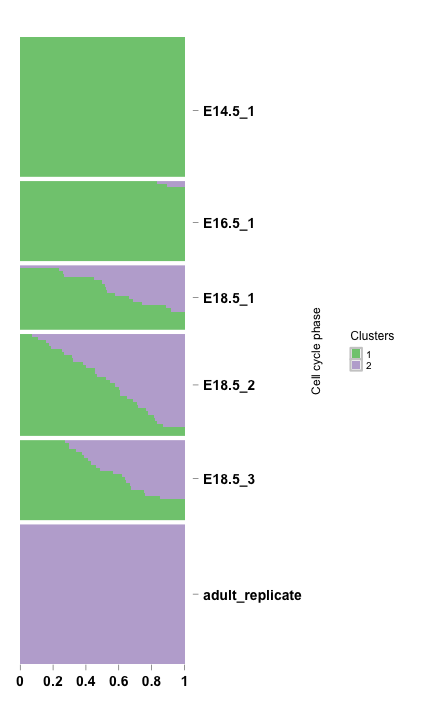
\includegraphics[width=3 in,height=5 in]{figure/structure_treutlin_classtpx_omega_fix-1} 

\end{knitrout}

We perform the method with \begin{verb} theta.fix() \end{verb} for K=2 and K=3.

\begin{knitrout}
\definecolor{shadecolor}{rgb}{0.969, 0.969, 0.969}\color{fgcolor}\begin{kframe}
\begin{alltt}
\hlstd{Topic_clus} \hlkwb{<-} \hlstd{classtpx}\hlopt{::}\hlkwd{class_topics}\hlstd{(}
    \hlstd{counts_data,}
    \hlkwc{K}\hlstd{=}\hlnum{2}\hlstd{,}
    \hlkwc{known_samples} \hlstd{= known_samples,}
    \hlkwc{class_labs} \hlstd{= class_labs,}
    \hlkwc{method}\hlstd{=}\hlstr{"theta.fix"}\hlstd{,}
    \hlkwc{tol}\hlstd{=}\hlnum{0.01}\hlstd{,}
    \hlkwc{shrink}\hlstd{=}\hlnum{FALSE}\hlstd{)}

\hlkwd{save}\hlstd{(Topic_clus,} \hlkwc{file}\hlstd{=}\hlstr{"../rdas/treutlin_topic_fit_2_classtpx_theta_fix.rda"}\hlstd{)}
\end{alltt}
\end{kframe}
\end{knitrout}

\begin{knitrout}
\definecolor{shadecolor}{rgb}{0.969, 0.969, 0.969}\color{fgcolor}\begin{kframe}
\begin{alltt}
\hlstd{Topic_clus} \hlkwb{<-} \hlkwd{get}\hlstd{(}\hlkwd{load}\hlstd{(}\hlkwc{file}\hlstd{=}\hlstr{"../data/treutlin_topic_fit_2_classtpx_theta_fix.rda"}\hlstd{))}

\hlstd{omega} \hlkwb{<-} \hlstd{Topic_clus}\hlopt{$}\hlstd{omega;}

\hlstd{annotation} \hlkwb{<-} \hlkwd{data.frame}\hlstd{(}
  \hlkwc{sample_id} \hlstd{=} \hlkwd{paste0}\hlstd{(}\hlstr{"X"}\hlstd{,} \hlkwd{c}\hlstd{(}\hlnum{1}\hlopt{:}\hlkwd{NROW}\hlstd{(omega))),}
  \hlkwc{tissue_label} \hlstd{=} \hlkwd{factor}\hlstd{(}\hlkwd{paste0}\hlstd{(pheno_metadata}\hlopt{$}\hlstd{cell_type,} \hlstr{"_"}\hlstd{,}
                               \hlstd{pheno_metadata}\hlopt{$}\hlstd{replicate),}
                        \hlkwc{levels}\hlstd{=}\hlkwd{rev}\hlstd{(}\hlkwd{c}\hlstd{(}\hlstr{"E14.5_1"}\hlstd{,} \hlstr{"E16.5_1"}\hlstd{,}
                                     \hlstr{"E18.5_1"}\hlstd{,}\hlstr{"E18.5_2"}\hlstd{,}
                                     \hlstr{"E18.5_3"}\hlstd{,}\hlstr{"adult_replicate"}\hlstd{))}
\hlstd{))}

\hlkwd{rownames}\hlstd{(omega)} \hlkwb{<-} \hlstd{annotation}\hlopt{$}\hlstd{sample_id;}


\hlstd{CountClust}\hlopt{::}\hlkwd{StructureGGplot}\hlstd{(}\hlkwc{omega} \hlstd{= omega,}
                \hlkwc{annotation} \hlstd{= annotation,}
                \hlkwc{palette} \hlstd{= RColorBrewer}\hlopt{::}\hlkwd{brewer.pal}\hlstd{(}\hlnum{8}\hlstd{,} \hlstr{"Accent"}\hlstd{),}
                \hlkwc{yaxis_label} \hlstd{=} \hlstr{"Cell cycle phase"}\hlstd{,}
                \hlkwc{order_sample} \hlstd{=} \hlnum{TRUE}\hlstd{,}
                \hlkwc{axis_tick} \hlstd{=} \hlkwd{list}\hlstd{(}\hlkwc{axis_ticks_length} \hlstd{=} \hlnum{.1}\hlstd{,}
                                 \hlkwc{axis_ticks_lwd_y} \hlstd{=} \hlnum{.1}\hlstd{,}
                                 \hlkwc{axis_ticks_lwd_x} \hlstd{=} \hlnum{.1}\hlstd{,}
                                 \hlkwc{axis_label_size} \hlstd{=} \hlnum{7}\hlstd{,}
                                 \hlkwc{axis_label_face} \hlstd{=} \hlstr{"bold"}\hlstd{))}
\end{alltt}
\end{kframe}
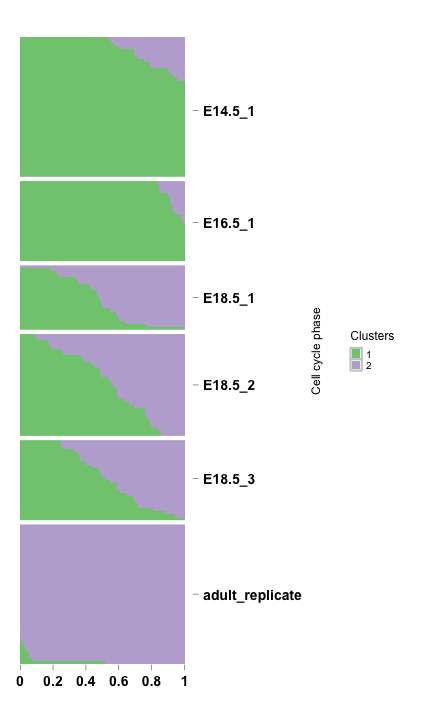
\includegraphics[width=3 in,height=5 in]{figure/structure_treutlin_classtpx_theta_fix_2-1} 

\end{knitrout}

\begin{knitrout}
\definecolor{shadecolor}{rgb}{0.969, 0.969, 0.969}\color{fgcolor}\begin{kframe}
\begin{alltt}
\hlstd{Topic_clus} \hlkwb{<-} \hlstd{classtpx}\hlopt{::}\hlkwd{class_topics}\hlstd{(}
    \hlstd{counts_data,}
    \hlkwc{K}\hlstd{=}\hlnum{2}\hlstd{,}
    \hlkwc{known_samples} \hlstd{= known_samples,}
    \hlkwc{class_labs} \hlstd{= class_labs,}
    \hlkwc{method}\hlstd{=}\hlstr{"theta.fix"}\hlstd{,}
    \hlkwc{tol}\hlstd{=}\hlnum{0.01}\hlstd{,}
    \hlkwc{shrink}\hlstd{=}\hlnum{FALSE}\hlstd{)}

\hlkwd{save}\hlstd{(Topic_clus,} \hlkwc{file}\hlstd{=}\hlstr{"../data/treutlin_topic_fit_3_classtpx_theta_fix.rda"}\hlstd{)}
\end{alltt}
\end{kframe}
\end{knitrout}

\begin{knitrout}
\definecolor{shadecolor}{rgb}{0.969, 0.969, 0.969}\color{fgcolor}\begin{kframe}
\begin{alltt}
\hlstd{Topic_clus} \hlkwb{<-} \hlkwd{get}\hlstd{(}\hlkwd{load}\hlstd{(}\hlkwc{file}\hlstd{=}\hlstr{"../data/treutlin_topic_fit_3_classtpx_theta_fix.rda"}\hlstd{))}

\hlstd{omega} \hlkwb{<-} \hlstd{Topic_clus}\hlopt{$}\hlstd{omega;}

\hlstd{annotation} \hlkwb{<-} \hlkwd{data.frame}\hlstd{(}
  \hlkwc{sample_id} \hlstd{=} \hlkwd{paste0}\hlstd{(}\hlstr{"X"}\hlstd{,} \hlkwd{c}\hlstd{(}\hlnum{1}\hlopt{:}\hlkwd{NROW}\hlstd{(omega))),}
  \hlkwc{tissue_label} \hlstd{=} \hlkwd{factor}\hlstd{(}\hlkwd{paste0}\hlstd{(pheno_metadata}\hlopt{$}\hlstd{cell_type,} \hlstr{"_"}\hlstd{,}
                               \hlstd{pheno_metadata}\hlopt{$}\hlstd{replicate),}
                        \hlkwc{levels}\hlstd{=}\hlkwd{rev}\hlstd{(}\hlkwd{c}\hlstd{(}\hlstr{"E14.5_1"}\hlstd{,} \hlstr{"E16.5_1"}\hlstd{,}
                                     \hlstr{"E18.5_1"}\hlstd{,}\hlstr{"E18.5_2"}\hlstd{,}
                                     \hlstr{"E18.5_3"}\hlstd{,}\hlstr{"adult_replicate"}\hlstd{))}
\hlstd{))}

\hlkwd{rownames}\hlstd{(omega)} \hlkwb{<-} \hlstd{annotation}\hlopt{$}\hlstd{sample_id;}


\hlstd{CountClust}\hlopt{::}\hlkwd{StructureGGplot}\hlstd{(}\hlkwc{omega} \hlstd{= omega,}
                \hlkwc{annotation} \hlstd{= annotation,}
                \hlkwc{palette} \hlstd{= RColorBrewer}\hlopt{::}\hlkwd{brewer.pal}\hlstd{(}\hlnum{8}\hlstd{,} \hlstr{"Accent"}\hlstd{),}
                \hlkwc{yaxis_label} \hlstd{=} \hlstr{"Cell cycle phase"}\hlstd{,}
                \hlkwc{order_sample} \hlstd{=} \hlnum{TRUE}\hlstd{,}
                \hlkwc{axis_tick} \hlstd{=} \hlkwd{list}\hlstd{(}\hlkwc{axis_ticks_length} \hlstd{=} \hlnum{.1}\hlstd{,}
                                 \hlkwc{axis_ticks_lwd_y} \hlstd{=} \hlnum{.1}\hlstd{,}
                                 \hlkwc{axis_ticks_lwd_x} \hlstd{=} \hlnum{.1}\hlstd{,}
                                 \hlkwc{axis_label_size} \hlstd{=} \hlnum{7}\hlstd{,}
                                 \hlkwc{axis_label_face} \hlstd{=} \hlstr{"bold"}\hlstd{))}
\end{alltt}
\end{kframe}
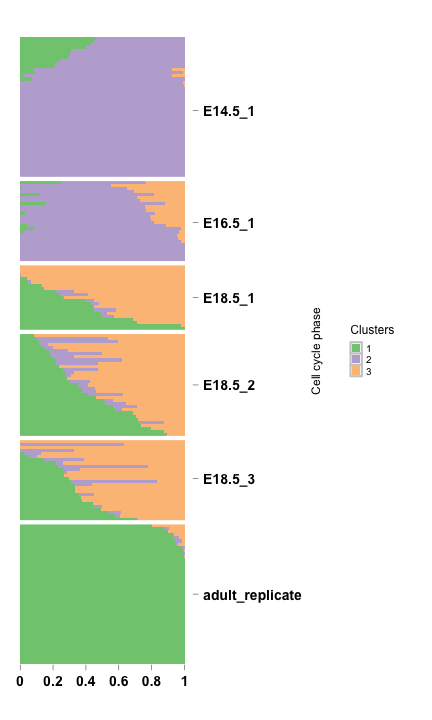
\includegraphics[width=3 in,height=5 in]{figure/structure_treutlin_classtpx_theta_fix_3-1} 

\end{knitrout}

\subsection{Scialdone et al (2015)}

Scialdone et al sequenced bulk-FACS sorted cells from phases G1, S and G2M phases. Also they sequenced a number of liver cells and they showed from PCA analysis that most of these liver cells seemed close to the G1 phase data. This was intuitive as most of these differentiated liver cells are in G1 phase. We perform classtpx here on the liver cells taking the bulk-RNA FACS sorted data from G1, S and G2M phases to represent three classes or clusters.

\begin{knitrout}
\definecolor{shadecolor}{rgb}{0.969, 0.969, 0.969}\color{fgcolor}\begin{kframe}
\begin{alltt}
\hlstd{devtools}\hlopt{::}\hlkwd{install_github}\hlstd{(}\hlstr{"jhsiao999/singleCellRNASeqMouseScialdoneLiver"}\hlstd{,}
                         \hlkwc{force}\hlstd{=}\hlnum{TRUE}\hlstd{);}
\end{alltt}
\end{kframe}
\end{knitrout}

\begin{knitrout}
\definecolor{shadecolor}{rgb}{0.969, 0.969, 0.969}\color{fgcolor}\begin{kframe}
\begin{alltt}
\hlkwd{library}\hlstd{(singleCellRNASeqMouseScialdoneLiver)}
\hlkwd{data}\hlstd{(}\hlstr{"MouseScialdoneLiver"}\hlstd{)}
\hlstd{liver_data} \hlkwb{<-} \hlkwd{t}\hlstd{(Biobase}\hlopt{::}\hlkwd{exprs}\hlstd{(MouseScialdoneLiver));}
\end{alltt}
\end{kframe}
\end{knitrout}

Now we install the bulk FACS sorted cell cycle data from Scialdone et al (2015).

\begin{knitrout}
\definecolor{shadecolor}{rgb}{0.969, 0.969, 0.969}\color{fgcolor}\begin{kframe}
\begin{alltt}
\hlstd{devtools}\hlopt{::}\hlkwd{install_github}\hlstd{(}\hlstr{"jhsiao999/bulkRNASeqMouseScialdoneESC"}\hlstd{,} \hlkwc{force}\hlstd{=}\hlnum{TRUE}\hlstd{);}
\end{alltt}
\end{kframe}
\end{knitrout}

\begin{knitrout}
\definecolor{shadecolor}{rgb}{0.969, 0.969, 0.969}\color{fgcolor}\begin{kframe}
\begin{alltt}
\hlkwd{library}\hlstd{(bulkRNASeqMouseScialdoneESC)}
\hlkwd{data}\hlstd{(}\hlstr{"MouseScialdoneESC"}\hlstd{)}
\hlstd{facs_data} \hlkwb{<-} \hlkwd{t}\hlstd{(Biobase}\hlopt{::}\hlkwd{exprs}\hlstd{(MouseScialdoneESC));}
\hlstd{facs_pheno_metadata} \hlkwb{<-} \hlkwd{pData}\hlstd{(MouseScialdoneESC);}
\end{alltt}
\end{kframe}
\end{knitrout}

\begin{knitrout}
\definecolor{shadecolor}{rgb}{0.969, 0.969, 0.969}\color{fgcolor}\begin{kframe}
\begin{alltt}
\hlstd{indices_intersect} \hlkwb{<-} \hlkwd{intersect}\hlstd{(}\hlkwd{featureNames}\hlstd{(MouseScialdoneESC),}
                               \hlkwd{featureNames}\hlstd{(MouseScialdoneLiver))}

\hlstd{matched_liver} \hlkwb{<-}  \hlkwd{match}\hlstd{(indices_intersect,} \hlkwd{featureNames}\hlstd{(MouseScialdoneLiver))}
\hlstd{liver_data_mod} \hlkwb{<-} \hlstd{liver_data[,matched_liver];}
\hlkwd{colnames}\hlstd{(liver_data_mod)} \hlkwb{<-} \hlstd{indices_intersect;}

\hlstd{matched_facs} \hlkwb{<-} \hlkwd{match}\hlstd{(indices_intersect,} \hlkwd{featureNames}\hlstd{(MouseScialdoneESC))}
\hlstd{facs_data_mod} \hlkwb{<-} \hlstd{facs_data[,matched_facs];}
\hlkwd{colnames}\hlstd{(facs_data_mod)} \hlkwb{<-}  \hlstd{indices_intersect;}

\hlstd{counts} \hlkwb{<-} \hlkwd{rbind}\hlstd{(facs_data_mod, liver_data_mod);}
\end{alltt}
\end{kframe}
\end{knitrout}

We now fit the classtpx model with the first three samples (bulk FACS sorted data representing
cell cycle classes G1, S and G2M respectively) assumed to be from known classes.

\begin{knitrout}
\definecolor{shadecolor}{rgb}{0.969, 0.969, 0.969}\color{fgcolor}\begin{kframe}
\begin{alltt}
\hlstd{known_samples} \hlkwb{<-} \hlnum{1}\hlopt{:}\hlnum{3}\hlstd{;}
\hlstd{class_labs} \hlkwb{<-}  \hlnum{1}\hlopt{:}\hlnum{3}\hlstd{;}
\end{alltt}
\end{kframe}
\end{knitrout}

\begin{knitrout}
\definecolor{shadecolor}{rgb}{0.969, 0.969, 0.969}\color{fgcolor}\begin{kframe}
\begin{alltt}
\hlstd{Topic_clus} \hlkwb{<-} \hlstd{classtpx}\hlopt{::}\hlkwd{class_topics}\hlstd{(}
    \hlstd{counts,}
    \hlkwc{K}\hlstd{=}\hlnum{3}\hlstd{,}
    \hlkwc{known_samples} \hlstd{= known_samples,}
    \hlkwc{class_labs} \hlstd{= class_labs,}
    \hlkwc{method}\hlstd{=}\hlstr{"omega.fix"}\hlstd{,}
    \hlkwc{tol}\hlstd{=}\hlnum{0.01}\hlstd{,}
    \hlkwc{shrink}\hlstd{=}\hlnum{FALSE}\hlstd{)}

\hlkwd{save}\hlstd{(Topic_clus,} \hlkwc{file}\hlstd{=}\hlstr{"../data/scialdone_topic_fit_3_classtpx_omega_fix.rda"}\hlstd{)}
\end{alltt}
\end{kframe}
\end{knitrout}

\begin{knitrout}
\definecolor{shadecolor}{rgb}{0.969, 0.969, 0.969}\color{fgcolor}\begin{kframe}
\begin{alltt}
\hlstd{Topic_clus} \hlkwb{<-} \hlkwd{get}\hlstd{(}\hlkwd{load}\hlstd{(}\hlstr{"../data/scialdone_topic_fit_3_classtpx_omega_fix.rda"}\hlstd{))}
\hlstd{omega} \hlkwb{<-} \hlstd{Topic_clus}\hlopt{$}\hlstd{omega[}\hlopt{-}\hlstd{(}\hlnum{1}\hlopt{:}\hlnum{3}\hlstd{),];}

\hlstd{annotation} \hlkwb{<-} \hlkwd{data.frame}\hlstd{(}
  \hlkwc{sample_id} \hlstd{=} \hlkwd{paste0}\hlstd{(}\hlstr{"X"}\hlstd{,} \hlkwd{c}\hlstd{(}\hlnum{1}\hlopt{:}\hlkwd{NROW}\hlstd{(omega))),}
  \hlkwc{tissue_label} \hlstd{=} \hlkwd{factor}\hlstd{(}\hlkwd{as.character}\hlstd{(}\hlkwd{rep}\hlstd{(}\hlstr{"Liver"}\hlstd{,}\hlnum{96}\hlstd{)))}
\hlstd{)}

\hlkwd{rownames}\hlstd{(omega)} \hlkwb{<-} \hlstd{annotation}\hlopt{$}\hlstd{sample_id;}


\hlstd{CountClust}\hlopt{::}\hlkwd{StructureGGplot}\hlstd{(}\hlkwc{omega} \hlstd{= omega,}
                \hlkwc{annotation} \hlstd{= annotation,}
                \hlkwc{palette} \hlstd{= RColorBrewer}\hlopt{::}\hlkwd{brewer.pal}\hlstd{(}\hlnum{8}\hlstd{,} \hlstr{"Accent"}\hlstd{),}
                \hlkwc{yaxis_label} \hlstd{=} \hlstr{"Cell cycle phase"}\hlstd{,}
                \hlkwc{order_sample} \hlstd{=} \hlnum{TRUE}\hlstd{,}
                \hlkwc{axis_tick} \hlstd{=} \hlkwd{list}\hlstd{(}\hlkwc{axis_ticks_length} \hlstd{=} \hlnum{.1}\hlstd{,}
                                 \hlkwc{axis_ticks_lwd_y} \hlstd{=} \hlnum{.1}\hlstd{,}
                                 \hlkwc{axis_ticks_lwd_x} \hlstd{=} \hlnum{.1}\hlstd{,}
                                 \hlkwc{axis_label_size} \hlstd{=} \hlnum{7}\hlstd{,}
                                 \hlkwc{axis_label_face} \hlstd{=} \hlstr{"bold"}\hlstd{))}
\end{alltt}
\end{kframe}
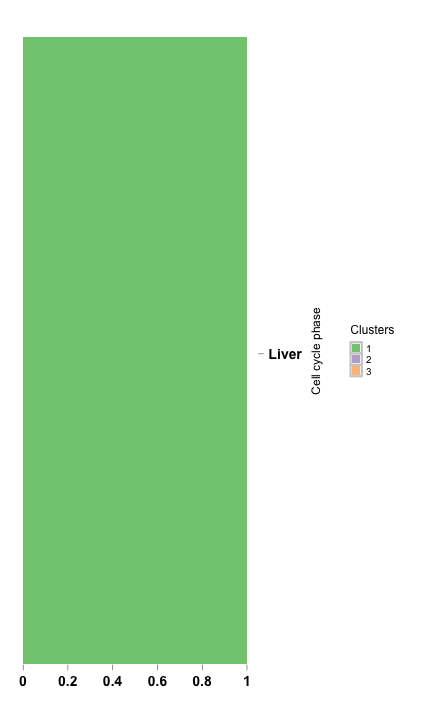
\includegraphics[width=3 in,height=5 in]{figure/structure_scialdone_classtpx_omega_fix_3-1} 

\end{knitrout}

Note that all the cells seem to be represented by the first class which corresponds to the G1 phase. We perform the same analysis with \begin{verb} theta.fix() \end{verb} method.

\begin{knitrout}
\definecolor{shadecolor}{rgb}{0.969, 0.969, 0.969}\color{fgcolor}\begin{kframe}
\begin{alltt}
\hlstd{Topic_clus} \hlkwb{<-} \hlstd{classtpx}\hlopt{::}\hlkwd{class_topics}\hlstd{(}
    \hlstd{counts,}
    \hlkwc{K}\hlstd{=}\hlnum{3}\hlstd{,}
    \hlkwc{known_samples} \hlstd{= known_samples,}
    \hlkwc{class_labs} \hlstd{= class_labs,}
    \hlkwc{method}\hlstd{=}\hlstr{"theta.fix"}\hlstd{,}
    \hlkwc{tol}\hlstd{=}\hlnum{0.01}\hlstd{,}
    \hlkwc{shrink}\hlstd{=}\hlnum{FALSE}\hlstd{)}

\hlkwd{save}\hlstd{(Topic_clus,} \hlkwc{file}\hlstd{=}\hlstr{"../data/scialdone_topic_fit_3_classtpx_theta_fix.rda"}\hlstd{)}
\end{alltt}
\end{kframe}
\end{knitrout}

\begin{knitrout}
\definecolor{shadecolor}{rgb}{0.969, 0.969, 0.969}\color{fgcolor}\begin{kframe}
\begin{alltt}
\hlstd{Topic_clus} \hlkwb{<-} \hlkwd{get}\hlstd{(}\hlkwd{load}\hlstd{(}\hlstr{"../data/scialdone_topic_fit_3_classtpx_theta_fix.rda"}\hlstd{))}
\hlstd{omega} \hlkwb{<-} \hlstd{Topic_clus}\hlopt{$}\hlstd{omega[}\hlopt{-}\hlstd{(}\hlnum{1}\hlopt{:}\hlnum{3}\hlstd{),];}

\hlstd{annotation} \hlkwb{<-} \hlkwd{data.frame}\hlstd{(}
  \hlkwc{sample_id} \hlstd{=} \hlkwd{paste0}\hlstd{(}\hlstr{"X"}\hlstd{,} \hlkwd{c}\hlstd{(}\hlnum{1}\hlopt{:}\hlkwd{NROW}\hlstd{(omega))),}
  \hlkwc{tissue_label} \hlstd{=} \hlkwd{factor}\hlstd{(}\hlkwd{as.character}\hlstd{(}\hlkwd{rep}\hlstd{(}\hlstr{"Liver"}\hlstd{,}\hlnum{96}\hlstd{)))}
\hlstd{)}

\hlkwd{rownames}\hlstd{(omega)} \hlkwb{<-} \hlstd{annotation}\hlopt{$}\hlstd{sample_id;}


\hlstd{CountClust}\hlopt{::}\hlkwd{StructureGGplot}\hlstd{(}\hlkwc{omega} \hlstd{= omega,}
                \hlkwc{annotation} \hlstd{= annotation,}
                \hlkwc{palette} \hlstd{= RColorBrewer}\hlopt{::}\hlkwd{brewer.pal}\hlstd{(}\hlnum{8}\hlstd{,} \hlstr{"Accent"}\hlstd{),}
                \hlkwc{yaxis_label} \hlstd{=} \hlstr{"Cell cycle phase"}\hlstd{,}
                \hlkwc{order_sample} \hlstd{=} \hlnum{TRUE}\hlstd{,}
                \hlkwc{axis_tick} \hlstd{=} \hlkwd{list}\hlstd{(}\hlkwc{axis_ticks_length} \hlstd{=} \hlnum{.1}\hlstd{,}
                                 \hlkwc{axis_ticks_lwd_y} \hlstd{=} \hlnum{.1}\hlstd{,}
                                 \hlkwc{axis_ticks_lwd_x} \hlstd{=} \hlnum{.1}\hlstd{,}
                                 \hlkwc{axis_label_size} \hlstd{=} \hlnum{7}\hlstd{,}
                                 \hlkwc{axis_label_face} \hlstd{=} \hlstr{"bold"}\hlstd{))}
\end{alltt}
\end{kframe}
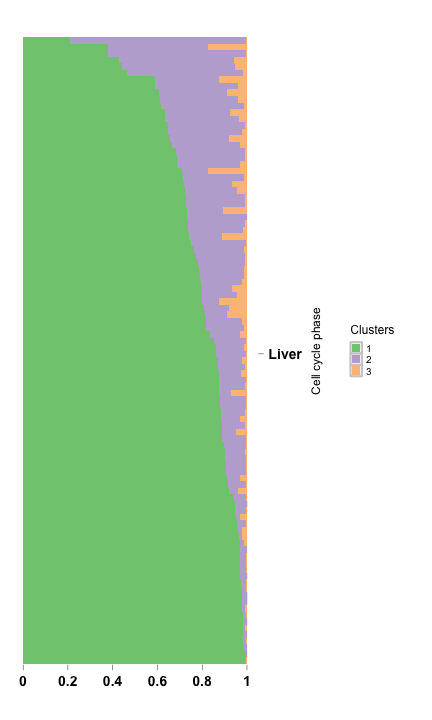
\includegraphics[width=3 in,height=5 in]{figure/structure_scialdone_classtpx_theta_fix_3-1} 

\end{knitrout}

Here also maximum representativeness is due to the cluster from G1 phase.

\subsection{Buettner et al 2015 + Leng et al 2015}

Buettner et al 2015 collected single cell RNA-seq FACS sorted data from cell cycle phases G1, G2 and S from mouse. Leng et al 2015 collected FACS sorted data from G1, G2 and S for humans. The idea was to see if we can use the FACS sorted mouse data coming from three cell cycle phases G1, G2 and S, to learn about human data and predict the cell cycle phases of the human data correctly.

The one barrier to doing so is that the genes in humans and those in mouse are different. But there are many ortholog genes which are common between the two species and we extract such genes out using BioMart. 

First we install and load the mouse single cell RNA-seq data due to Buettner et al 2015. 

\begin{knitrout}
\definecolor{shadecolor}{rgb}{0.969, 0.969, 0.969}\color{fgcolor}\begin{kframe}
\begin{alltt}
\hlstd{devtools}\hlopt{::}\hlkwd{install_github}\hlstd{(}\hlstr{"jhsiao999/singleCellRNASeqMouseBuettnerESC"}\hlstd{,} \hlkwc{force}\hlstd{=}\hlnum{TRUE}\hlstd{)}
\end{alltt}
\end{kframe}
\end{knitrout}

\begin{knitrout}
\definecolor{shadecolor}{rgb}{0.969, 0.969, 0.969}\color{fgcolor}\begin{kframe}
\begin{alltt}
\hlkwd{library}\hlstd{(singleCellRNASeqMouseBuettnerESC)}
\hlkwd{data}\hlstd{(}\hlstr{"MouseBuettnerESC"}\hlstd{)}
\hlstd{buettner_gene_names} \hlkwb{<-} \hlstd{Biobase}\hlopt{::}\hlkwd{featureNames}\hlstd{(MouseBuettnerESC);}

\hlstd{buettner_data} \hlkwb{<-} \hlstd{Biobase}\hlopt{::}\hlkwd{exprs}\hlstd{(MouseBuettnerESC);}
\hlstd{buettner_metadata} \hlkwb{<-} \hlstd{Biobase}\hlopt{::}\hlkwd{pData}\hlstd{(MouseBuettnerESC)}
\hlstd{buettner_cell_state} \hlkwb{<-} \hlstd{buettner_metadata}\hlopt{$}\hlstd{cell_cycle;}

\hlkwd{table}\hlstd{(buettner_cell_state)}
\end{alltt}
\begin{verbatim}
## buettner_cell_state
##  G1 G2M   S 
##  96  96  96
\end{verbatim}
\end{kframe}
\end{knitrout}

We now extract the ortholog genes common between the Leng et al 2015 data and the Buettner et al 2015 data.

\begin{knitrout}
\definecolor{shadecolor}{rgb}{0.969, 0.969, 0.969}\color{fgcolor}\begin{kframe}
\begin{alltt}
\hlkwd{library}\hlstd{(biomaRt)}
\hlstd{human} \hlkwb{=} \hlkwd{useMart}\hlstd{(}\hlstr{"ensembl"}\hlstd{,} \hlkwc{dataset} \hlstd{=} \hlstr{"hsapiens_gene_ensembl"}\hlstd{);}
\hlstd{attributes} \hlkwb{=} \hlkwd{c}\hlstd{(}\hlstr{"ensembl_gene_id"}\hlstd{,}\hlstr{"mmusculus_homolog_ensembl_gene"}\hlstd{,}
               \hlstr{"mmusculus_homolog_perc_id_r1"}\hlstd{)}
\hlstd{attributes}\hlkwb{=}\hlkwd{c}\hlstd{(attributes,}\hlstr{"mmusculus_homolog_orthology_type"}\hlstd{,}
\hlstr{"mmusculus_homolog_subtype"}\hlstd{,} \hlstr{"mmusculus_homolog_perc_id"}\hlstd{)}
\hlstd{orth.mouse.human} \hlkwb{=} \hlkwd{getBM}\hlstd{(attributes,}
\hlkwc{filters}\hlstd{=}\hlstr{"with_homolog_mmus"}\hlstd{,}\hlkwc{values}\hlstd{=}\hlnum{TRUE}\hlstd{,} \hlkwc{mart} \hlstd{= human,}
\hlkwc{uniqueRows}\hlstd{=}\hlnum{TRUE}\hlstd{)}
\end{alltt}
\end{kframe}
\end{knitrout}

We determine those ortholog human genes obtained above which have valid HGNC symbol 
which has been used to report feature names in the Leng et al 2015 data

\begin{knitrout}
\definecolor{shadecolor}{rgb}{0.969, 0.969, 0.969}\color{fgcolor}\begin{kframe}
\begin{alltt}
\hlstd{filter_indices} \hlkwb{<-} \hlkwd{match}\hlstd{(buettner_gene_names, orth.mouse.human[,}\hlnum{2}\hlstd{]);}
\hlstd{filter_indices} \hlkwb{<-} \hlstd{filter_indices[}\hlopt{!}\hlkwd{is.na}\hlstd{(filter_indices)];}
\hlstd{ortholog_buettner_mouse_ids} \hlkwb{<-} \hlstd{orth.mouse.human[filter_indices,}\hlnum{2}\hlstd{];}
\hlstd{ortholog_buettner_human_ids} \hlkwb{<-} \hlstd{orth.mouse.human[filter_indices,}\hlnum{1}\hlstd{];}

\hlstd{human} \hlkwb{=} \hlkwd{useMart}\hlstd{(}\hlstr{"ensembl"}\hlstd{,} \hlkwc{dataset} \hlstd{=} \hlstr{"hsapiens_gene_ensembl"}\hlstd{)}
\hlstd{mySymbols} \hlkwb{<-} \hlstd{ortholog_buettner_human_ids;} \hlcom{# mySymbols is a vector of MGI symbols.}
\hlstd{gene_list_human} \hlkwb{<-} \hlkwd{getBM}\hlstd{(} \hlkwc{attributes}\hlstd{=}\hlkwd{c}\hlstd{(}\hlstr{"ensembl_gene_id"}\hlstd{,} \hlstr{"hgnc_symbol"}\hlstd{) ,} \hlkwc{filters}\hlstd{=}
\hlstr{"ensembl_gene_id"}\hlstd{,} \hlkwc{values} \hlstd{=mySymbols ,}\hlkwc{mart}\hlstd{=human)}

\hlstd{gene_names_human} \hlkwb{<-} \hlstd{gene_list_human[,}\hlnum{2}\hlstd{];}
\end{alltt}
\end{kframe}
\end{knitrout}

We filter the Leng et al data

\begin{knitrout}
\definecolor{shadecolor}{rgb}{0.969, 0.969, 0.969}\color{fgcolor}\begin{kframe}
\begin{alltt}
\hlstd{matched_human_gene_indices_leng} \hlkwb{<-} \hlkwd{match}\hlstd{(gene_names_human, leng_gene_names)}
\hlstd{matched_human_gene_indices_leng} \hlkwb{<-}
  \hlstd{matched_human_gene_indices_leng[}\hlopt{!}\hlkwd{is.na}\hlstd{(matched_human_gene_indices_leng)];}


\hlstd{matched_genes_leng} \hlkwb{<-} \hlstd{leng_gene_names[matched_human_gene_indices_leng];}

\hlstd{filter_indices} \hlkwb{<-} \hlkwd{match}\hlstd{(matched_genes_leng, leng_gene_names);}

\hlstd{leng_filtered_data} \hlkwb{<-} \hlstd{leng_data[,filter_indices];}
\end{alltt}
\end{kframe}
\end{knitrout}

Next we filter the Buettner et al data

\begin{knitrout}
\definecolor{shadecolor}{rgb}{0.969, 0.969, 0.969}\color{fgcolor}\begin{kframe}
\begin{alltt}
\hlstd{filter_indices} \hlkwb{<-} \hlkwd{match}\hlstd{(gene_names_human, leng_gene_names);}
\hlstd{gene_list_human_filtered} \hlkwb{<-} \hlstd{gene_list_human[}\hlkwd{which}\hlstd{(}\hlopt{!}\hlkwd{is.na}\hlstd{(filter_indices)),];}
\hlstd{gene_names_human_filtered} \hlkwb{<-} \hlstd{gene_list_human_filtered[,}\hlnum{1}\hlstd{];}
\hlstd{human_ids_buettner} \hlkwb{<-}
  \hlstd{ortholog_buettner_human_ids[}\hlkwd{match}\hlstd{(gene_names_human_filtered,}
                                    \hlstd{ortholog_buettner_human_ids)];}
\hlstd{mouse_ortholog_ids_buettner} \hlkwb{<-}
  \hlstd{ortholog_buettner_mouse_ids[}\hlkwd{match}\hlstd{(gene_names_human_filtered,}
                                    \hlstd{ortholog_buettner_human_ids)];}

\hlstd{filter_genes_buettner} \hlkwb{<-} \hlkwd{match}\hlstd{(mouse_ortholog_ids_buettner, buettner_gene_names);}

\hlstd{buettner_filtered_data} \hlkwb{<-} \hlkwd{t}\hlstd{(buettner_data[filter_genes_buettner,]);}
\end{alltt}
\end{kframe}
\end{knitrout}

We pool the filtered data from Leng et al and Buettner et al containing expression patterns of ortholog matched genes.

\begin{knitrout}
\definecolor{shadecolor}{rgb}{0.969, 0.969, 0.969}\color{fgcolor}\begin{kframe}
\begin{alltt}
\hlstd{pooled_data} \hlkwb{<-} \hlkwd{rbind}\hlstd{(buettner_filtered_data, leng_filtered_data);}
\end{alltt}
\end{kframe}
\end{knitrout}

We first apply the \begin{verb} topics() \end{verb} of the \begin{verb} maptpx() \end{verb} package to detrmine the unsupervised clustering patterns. 

\begin{knitrout}
\definecolor{shadecolor}{rgb}{0.969, 0.969, 0.969}\color{fgcolor}\begin{kframe}
\begin{alltt}
\hlstd{Topic_clus} \hlkwb{<-} \hlstd{maptpx}\hlopt{::}\hlkwd{topics}\hlstd{(}
    \hlstd{pooled_data,}
    \hlkwc{K}\hlstd{=}\hlnum{3}\hlstd{,}
    \hlkwc{tol}\hlstd{=}\hlnum{0.1}
    \hlstd{)}

\hlkwd{save}\hlstd{(Topic_clus,} \hlkwc{file}\hlstd{=}\hlstr{"../data/leng_topic_fit_3_maptpx_buettner.rda"}\hlstd{)}
\end{alltt}
\end{kframe}
\end{knitrout}

\begin{knitrout}
\definecolor{shadecolor}{rgb}{0.969, 0.969, 0.969}\color{fgcolor}\begin{kframe}
\begin{alltt}
\hlstd{Topic_clus} \hlkwb{<-} \hlkwd{get}\hlstd{(}\hlkwd{load}\hlstd{(}\hlkwc{file}\hlstd{=}\hlstr{"../data/leng_topic_fit_3_maptpx_buettner.rda"}\hlstd{))}

\hlstd{omega} \hlkwb{<-} \hlstd{Topic_clus}\hlopt{$}\hlstd{omega;}

\hlstd{leng_cell_state_human} \hlkwb{<-} \hlkwd{paste0}\hlstd{(}\hlstr{"human"}\hlstd{,} \hlstr{"_"}\hlstd{, leng_cell_state);}
\hlstd{buettner_cell_state_mouse} \hlkwb{<-} \hlkwd{paste0}\hlstd{(}\hlstr{"mouse"}\hlstd{,}\hlstr{"_"}\hlstd{, buettner_cell_state);}

\hlstd{annotation} \hlkwb{<-} \hlkwd{data.frame}\hlstd{(}
  \hlkwc{sample_id} \hlstd{=} \hlkwd{paste0}\hlstd{(}\hlstr{"X"}\hlstd{,} \hlkwd{c}\hlstd{(}\hlnum{1}\hlopt{:}\hlkwd{NROW}\hlstd{(omega))),}
  \hlkwc{tissue_label} \hlstd{=} \hlkwd{factor}\hlstd{(}\hlkwd{c}\hlstd{(}\hlkwd{as.character}\hlstd{(buettner_cell_state_mouse),}
                          \hlkwd{as.character}\hlstd{(leng_cell_state_human)),}
                        \hlkwc{levels} \hlstd{=} \hlkwd{c}\hlstd{(}\hlstr{"mouse_G1"}\hlstd{,} \hlstr{"mouse_S"}\hlstd{,} \hlstr{"mouse_G2M"}\hlstd{,}
                                        \hlstr{"human_G1"}\hlstd{,}\hlstr{"human_S"}\hlstd{,}
                                         \hlstr{"human_G2"}\hlstd{,} \hlstr{"human_H1"}\hlstd{) ) )}


\hlkwd{rownames}\hlstd{(omega)} \hlkwb{<-} \hlstd{annotation}\hlopt{$}\hlstd{sample_id;}


\hlstd{CountClust}\hlopt{::}\hlkwd{StructureGGplot}\hlstd{(}\hlkwc{omega} \hlstd{= omega,}
                \hlkwc{annotation} \hlstd{= annotation,}
                \hlkwc{palette} \hlstd{= RColorBrewer}\hlopt{::}\hlkwd{brewer.pal}\hlstd{(}\hlnum{8}\hlstd{,} \hlstr{"Accent"}\hlstd{),}
                \hlkwc{yaxis_label} \hlstd{=} \hlstr{"Cell cycle phase"}\hlstd{,}
                \hlkwc{order_sample} \hlstd{=} \hlnum{TRUE}\hlstd{,}
                \hlkwc{axis_tick} \hlstd{=} \hlkwd{list}\hlstd{(}\hlkwc{axis_ticks_length} \hlstd{=} \hlnum{.1}\hlstd{,}
                                 \hlkwc{axis_ticks_lwd_y} \hlstd{=} \hlnum{.1}\hlstd{,}
                                 \hlkwc{axis_ticks_lwd_x} \hlstd{=} \hlnum{.1}\hlstd{,}
                                 \hlkwc{axis_label_size} \hlstd{=} \hlnum{7}\hlstd{,}
                                 \hlkwc{axis_label_face} \hlstd{=} \hlstr{"bold"}\hlstd{))}
\end{alltt}
\end{kframe}
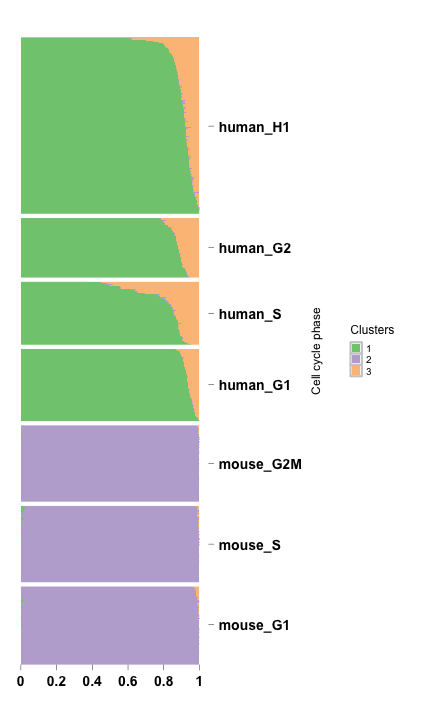
\includegraphics[width=3 in,height=5 in]{figure/structure_ortholog_maptpx-1} 

\end{knitrout}

Note that when the clustering is performed over mouse and human ortholog genes together, it seems to pick up those genes that separate the two species rather than finding out cell-cycle related structure. This is again more intuitive I guess as the inter species differences are way stronger than the cell cycle effect. 

We next performed classtpx model by using the mouse data as training sample and we fit $K=3$ model with both \begin{verb} omega.fix() \end{verb} and \begin{verb} theta.fix() \end{verb} methods.

\begin{knitrout}
\definecolor{shadecolor}{rgb}{0.969, 0.969, 0.969}\color{fgcolor}\begin{kframe}
\begin{alltt}
\hlstd{known_samples} \hlkwb{<-} \hlnum{1}\hlopt{:}\hlnum{288}\hlstd{;}
\hlstd{class_labs} \hlkwb{<-} \hlkwd{c}\hlstd{(}\hlkwd{rep}\hlstd{(}\hlnum{1}\hlstd{,}\hlnum{96}\hlstd{),} \hlkwd{rep}\hlstd{(}\hlnum{2}\hlstd{,}\hlnum{96}\hlstd{),} \hlkwd{rep}\hlstd{(}\hlnum{3}\hlstd{,}\hlnum{96}\hlstd{));}
\end{alltt}
\end{kframe}
\end{knitrout}

\begin{knitrout}
\definecolor{shadecolor}{rgb}{0.969, 0.969, 0.969}\color{fgcolor}\begin{kframe}
\begin{alltt}
\hlstd{Topic_clus} \hlkwb{<-} \hlstd{classtpx}\hlopt{::}\hlkwd{class_topics}\hlstd{(}
    \hlstd{counts,}
    \hlkwc{K}\hlstd{=}\hlnum{3}\hlstd{,}
    \hlkwc{known_samples} \hlstd{= known_samples,}
    \hlkwc{class_labs} \hlstd{= class_labs,}
    \hlkwc{method}\hlstd{=}\hlstr{"omega.fix"}\hlstd{,}
    \hlkwc{tol}\hlstd{=}\hlnum{0.01}\hlstd{,}
    \hlkwc{shrink}\hlstd{=}\hlnum{FALSE}\hlstd{)}

\hlkwd{save}\hlstd{(Topic_clus,} \hlkwc{file}\hlstd{=}\hlstr{"../data/leng_topic_fit_classtpx_omega_fix_buettner.rda"}\hlstd{)}
\end{alltt}
\end{kframe}
\end{knitrout}

\begin{knitrout}
\definecolor{shadecolor}{rgb}{0.969, 0.969, 0.969}\color{fgcolor}\begin{kframe}
\begin{alltt}
\hlstd{Topic_clus} \hlkwb{<-} \hlkwd{get}\hlstd{(}\hlkwd{load}\hlstd{(}\hlstr{"../data/leng_topic_fit_classtpx_omega_fix_buettner.rda"}\hlstd{))}
\hlstd{omega} \hlkwb{<-} \hlstd{Topic_clus}\hlopt{$}\hlstd{omega;}

\hlstd{leng_cell_state_human} \hlkwb{<-} \hlkwd{paste0}\hlstd{(}\hlstr{"human"}\hlstd{,} \hlstr{"_"}\hlstd{, leng_cell_state);}
\hlstd{buettner_cell_state_mouse} \hlkwb{<-} \hlkwd{paste0}\hlstd{(}\hlstr{"mouse"}\hlstd{,}\hlstr{"_"}\hlstd{, buettner_cell_state);}

\hlstd{annotation} \hlkwb{<-} \hlkwd{data.frame}\hlstd{(}
  \hlkwc{sample_id} \hlstd{=} \hlkwd{paste0}\hlstd{(}\hlstr{"X"}\hlstd{,} \hlkwd{c}\hlstd{(}\hlnum{1}\hlopt{:}\hlkwd{NROW}\hlstd{(omega))),}
  \hlkwc{tissue_label} \hlstd{=} \hlkwd{factor}\hlstd{(}\hlkwd{c}\hlstd{(}\hlkwd{as.character}\hlstd{(buettner_cell_state_mouse),}
                          \hlkwd{as.character}\hlstd{(leng_cell_state_human)),}
                        \hlkwc{levels} \hlstd{=} \hlkwd{c}\hlstd{(}\hlstr{"mouse_G1"}\hlstd{,} \hlstr{"mouse_S"}\hlstd{,} \hlstr{"mouse_G2M"}\hlstd{,}
                                        \hlstr{"human_G1"}\hlstd{,}\hlstr{"human_S"}\hlstd{,}
                                         \hlstr{"human_G2"}\hlstd{,} \hlstr{"human_H1"}\hlstd{) ) )}


\hlkwd{rownames}\hlstd{(omega)} \hlkwb{<-} \hlstd{annotation}\hlopt{$}\hlstd{sample_id;}


\hlstd{CountClust}\hlopt{::}\hlkwd{StructureGGplot}\hlstd{(}\hlkwc{omega} \hlstd{= omega,}
                \hlkwc{annotation} \hlstd{= annotation,}
                \hlkwc{palette} \hlstd{= RColorBrewer}\hlopt{::}\hlkwd{brewer.pal}\hlstd{(}\hlnum{8}\hlstd{,} \hlstr{"Accent"}\hlstd{),}
                \hlkwc{yaxis_label} \hlstd{=} \hlstr{"Cell cycle phase"}\hlstd{,}
                \hlkwc{order_sample} \hlstd{=} \hlnum{TRUE}\hlstd{,}
                \hlkwc{axis_tick} \hlstd{=} \hlkwd{list}\hlstd{(}\hlkwc{axis_ticks_length} \hlstd{=} \hlnum{.1}\hlstd{,}
                                 \hlkwc{axis_ticks_lwd_y} \hlstd{=} \hlnum{.1}\hlstd{,}
                                 \hlkwc{axis_ticks_lwd_x} \hlstd{=} \hlnum{.1}\hlstd{,}
                                 \hlkwc{axis_label_size} \hlstd{=} \hlnum{7}\hlstd{,}
                                 \hlkwc{axis_label_face} \hlstd{=} \hlstr{"bold"}\hlstd{))}
\end{alltt}
\end{kframe}
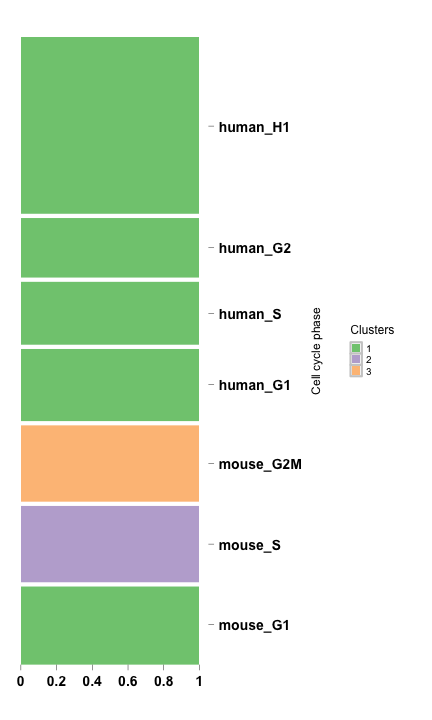
\includegraphics[width=3 in,height=5 in]{figure/structure_ortholog_classtpx_omega_fix_3-1} 

\end{knitrout}

\begin{knitrout}
\definecolor{shadecolor}{rgb}{0.969, 0.969, 0.969}\color{fgcolor}\begin{kframe}
\begin{alltt}
\hlstd{Topic_clus} \hlkwb{<-} \hlstd{classtpx}\hlopt{::}\hlkwd{class_topics}\hlstd{(}
    \hlstd{pooled_data,}
    \hlkwc{K}\hlstd{=}\hlnum{3}\hlstd{,}
    \hlkwc{known_samples} \hlstd{= known_samples,}
    \hlkwc{class_labs} \hlstd{= class_labs,}
    \hlkwc{method}\hlstd{=}\hlstr{"theta.fix"}\hlstd{,}
    \hlkwc{tol}\hlstd{=}\hlnum{0.01}\hlstd{,}
    \hlkwc{shrink}\hlstd{=}\hlnum{FALSE}\hlstd{)}

\hlkwd{save}\hlstd{(Topic_clus,} \hlkwc{file}\hlstd{=}\hlstr{"../data/leng_topic_fit_classtpx_theta_fix_buettner.rda"}\hlstd{)}
\end{alltt}
\end{kframe}
\end{knitrout}

\begin{knitrout}
\definecolor{shadecolor}{rgb}{0.969, 0.969, 0.969}\color{fgcolor}\begin{kframe}
\begin{alltt}
\hlstd{Topic_clus} \hlkwb{<-} \hlkwd{get}\hlstd{(}\hlkwd{load}\hlstd{(}\hlstr{"../data/leng_topic_fit_classtpx_theta_fix_buettner.rda"}\hlstd{))}
\hlstd{omega} \hlkwb{<-} \hlstd{Topic_clus}\hlopt{$}\hlstd{omega;}

\hlstd{leng_cell_state_human} \hlkwb{<-} \hlkwd{paste0}\hlstd{(}\hlstr{"human"}\hlstd{,} \hlstr{"_"}\hlstd{, leng_cell_state);}
\hlstd{buettner_cell_state_mouse} \hlkwb{<-} \hlkwd{paste0}\hlstd{(}\hlstr{"mouse"}\hlstd{,}\hlstr{"_"}\hlstd{, buettner_cell_state);}

\hlstd{annotation} \hlkwb{<-} \hlkwd{data.frame}\hlstd{(}
  \hlkwc{sample_id} \hlstd{=} \hlkwd{paste0}\hlstd{(}\hlstr{"X"}\hlstd{,} \hlkwd{c}\hlstd{(}\hlnum{1}\hlopt{:}\hlkwd{NROW}\hlstd{(omega))),}
  \hlkwc{tissue_label} \hlstd{=} \hlkwd{factor}\hlstd{(}\hlkwd{c}\hlstd{(}\hlkwd{as.character}\hlstd{(buettner_cell_state_mouse),}
                          \hlkwd{as.character}\hlstd{(leng_cell_state_human)),}
                        \hlkwc{levels} \hlstd{=} \hlkwd{c}\hlstd{(}\hlstr{"mouse_G1"}\hlstd{,} \hlstr{"mouse_S"}\hlstd{,} \hlstr{"mouse_G2M"}\hlstd{,}
                                        \hlstr{"human_G1"}\hlstd{,}\hlstr{"human_S"}\hlstd{,}
                                         \hlstr{"human_G2"}\hlstd{,} \hlstr{"human_H1"}\hlstd{) ) )}


\hlkwd{rownames}\hlstd{(omega)} \hlkwb{<-} \hlstd{annotation}\hlopt{$}\hlstd{sample_id;}


\hlstd{CountClust}\hlopt{::}\hlkwd{StructureGGplot}\hlstd{(}\hlkwc{omega} \hlstd{= omega,}
                \hlkwc{annotation} \hlstd{= annotation,}
                \hlkwc{palette} \hlstd{= RColorBrewer}\hlopt{::}\hlkwd{brewer.pal}\hlstd{(}\hlnum{8}\hlstd{,} \hlstr{"Accent"}\hlstd{),}
                \hlkwc{yaxis_label} \hlstd{=} \hlstr{"Cell cycle phase"}\hlstd{,}
                \hlkwc{order_sample} \hlstd{=} \hlnum{TRUE}\hlstd{,}
                \hlkwc{axis_tick} \hlstd{=} \hlkwd{list}\hlstd{(}\hlkwc{axis_ticks_length} \hlstd{=} \hlnum{.1}\hlstd{,}
                                 \hlkwc{axis_ticks_lwd_y} \hlstd{=} \hlnum{.1}\hlstd{,}
                                 \hlkwc{axis_ticks_lwd_x} \hlstd{=} \hlnum{.1}\hlstd{,}
                                 \hlkwc{axis_label_size} \hlstd{=} \hlnum{7}\hlstd{,}
                                 \hlkwc{axis_label_face} \hlstd{=} \hlstr{"bold"}\hlstd{))}
\end{alltt}
\end{kframe}
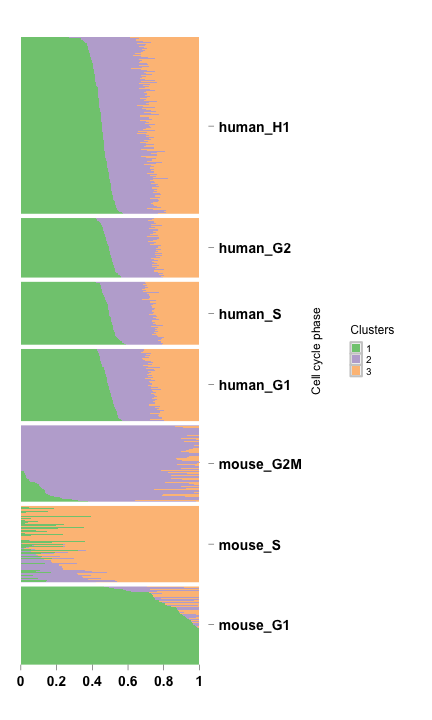
\includegraphics[width=3 in,height=5 in]{figure/structure_ortholog_classtpx_theta_fix_3-1} 

\end{knitrout}

The above analysis (especially for the \begin{verb} theta.fix \end{verb} approach) shows that the cluster patterns obtained from cell cycle phases of mouse does not quite explain the patterns in the human data. One reason could be because we have pooled all the ortholog genes in this analysis
and not just the cell-cycle related genes. It could also mean the orthologs of cell-cycle genes for mouse may not be cell-cycle related genes for humans.

\section{Discussion}

\begin{itemize}

\item Since the number of features (genes) is usually way larger than the number of samples in RNA-seq data, it is important to protect the analysis from noisy genes which are not informative biologically but incorporate a lot of variation that can compromise the results. We use the adaptive shrinkage method (check Methods and Materials) through \begin{verb} shrink=TRUE \end{verb} to effectively reweigh the variables based on their within-class variation. The shrinkage method adopted may be improved by using FASH due to Mengyin Lu \url{https://github.com/mengyin/ashlar-fash}. Her model shrinks the F-statistics derived from the following linear model (which may be applied on voom transformed data)

\begin{equation}
Y_{ng}=\mu_{g}+\beta_{cl(n),g}+e_{ng} \hspace{1 cm} \beta_{cl(n),g} \sim N(0, \sigma^2) \hspace{1 cm} e_{ng} \sim N(0, s^2)
\end{equation}

However I am not sure how I can go from shrunk F-statistics in this model to shrunk estimates 
of $\beta$ values, which I think is what I may need ultimately to obtain refined estimates of $\theta$.

\item We may want to indicate in the Structure plot visualization, which samples have known class labels and what that class label is, compared to the ones for which we have no information about class labels. This would be particularly handy in case of \begin{verb} theta.fix() \end{verb} or \begin{verb} theta.prior \end{verb} models where it is not clear just from viewing the Structure plot, which of the samples have known cluster memberships.

\item So far the attempt has been to take data from multiple experiments across labs and then check how far the knowledge of patterns from experiment in one lab can explain the patterns in the other. But there seems to be differences probably resulting from lab effects or batch or plate effects (cases in point: Buettner + Scialdone 2015 data analysis, Deng et al 2014 + Blakeley et al 2015 data analysis).

\item For additional simulated data and  real data applications of the \classtpx{} package, please check \textit{Cell classification using classtpx} section in \url{http://jhsiao999.github.io/singleCell-method/} and for codes and source files, please check: \url{https://github.com/kkdey/classtpx}.

\end{itemize}


\section{Session Info}

\begin{knitrout}
\definecolor{shadecolor}{rgb}{0.969, 0.969, 0.969}\color{fgcolor}\begin{kframe}
\begin{alltt}
\hlkwd{sessionInfo}\hlstd{()}
\end{alltt}
\begin{verbatim}
## R version 3.2.4 (2016-03-10)
## Platform: x86_64-apple-darwin13.4.0 (64-bit)
## Running under: OS X 10.10.5 (Yosemite)
## 
## locale:
## [1] en_US.UTF-8/en_US.UTF-8/en_US.UTF-8/C/en_US.UTF-8/en_US.UTF-8
## 
## attached base packages:
## [1] parallel  stats     graphics  grDevices utils     datasets  methods  
## [8] base     
## 
## other attached packages:
##  [1] biomaRt_2.26.1                            
##  [2] singleCellRNASeqMouseBuettnerESC_0.99.0   
##  [3] bulkRNASeqMouseScialdoneESC_0.99.0        
##  [4] singleCellRNASeqMouseScialdoneLiver_0.99.0
##  [5] singleCellRNASeqMouseTreutleinLung_0.99.0 
##  [6] singleCellRNASeqHumanLengESC_0.99.0       
##  [7] Biobase_2.30.0                            
##  [8] BiocGenerics_0.16.1                       
##  [9] classtpx_0.0.1                            
## [10] slam_0.1-32                               
## [11] knitr_1.12.3                              
## 
## loaded via a namespace (and not attached):
##  [1] Rcpp_0.12.3          formatR_1.2.1        RColorBrewer_1.1-2  
##  [4] plyr_1.8.3           highr_0.5.1          bitops_1.0-6        
##  [7] tools_3.2.4          digest_0.6.9         RSQLite_1.0.0       
## [10] evaluate_0.8         gtable_0.2.0         nlme_3.1-125        
## [13] lattice_0.20-33      mgcv_1.8-12          Matrix_1.2-4        
## [16] DBI_0.3.1            stringr_1.0.0        cluster_2.0.3       
## [19] IRanges_2.4.6        S4Vectors_0.8.7      gtools_3.5.0        
## [22] CountClust_0.99.3    stats4_3.2.4         grid_3.2.4          
## [25] nnet_7.3-12          cowplot_0.6.1        maptpx_1.9-2        
## [28] flexmix_2.3-13       AnnotationDbi_1.32.3 XML_3.98-1.3        
## [31] limma_3.26.8         ggplot2_2.1.0        reshape2_1.4.1      
## [34] magrittr_1.5         scales_0.4.0         modeltools_0.2-21   
## [37] MASS_7.3-45          BiocStyle_1.8.0      picante_1.6-2       
## [40] permute_0.9-0        colorspace_1.2-6     ape_3.4             
## [43] labeling_0.3         stringi_1.0-1        RCurl_1.95-4.7      
## [46] munsell_0.4.3        vegan_2.3-4
\end{verbatim}
\end{kframe}
\end{knitrout}

\end{document}
